\chapter{Portfolio}

\section{Sensor-Embedded Teeth for Oral Activity Recognition}

The human mouth is one part of the human body that is almost always in constant use. We use our mouth to perform some of the most important daily functions, such as eating, drinking, speaking, coughing, breathing, and smoking. Because our mouth is an opening into assessing the health of the human body, it presents the opportunity for the placement of a strategic sensor for detecting human oral activities. For this study, we developed such an oral sensory system, where we explored the use of a small motion sensor embedded inside artificial teeth for the recognition of human oral activities. The detection of human oral activities can enable numerous health care applications, such as food and fluid intake monitoring.   
Previous research has explored wearable sensory devices installed in various locations of the upper body for detecting human oral activities. For example, Amft et al. [1] used an earphone-attached microphone sensor to record human chewing sounds and detect food types based on their acoustic profiles. Amft et al. [2] proposed another approach that combined surface Electromyography (EMG) and a microphone worn around the neck area to recognize low- or high-volume swallowing actions. BodyScope [3] placed an acoustic sensor around the neck area to recognize different oral activities (e.g., eating, drinking, speaking, laughing, and coughing) by analyzing sounds generated from the throat area. In comparison, our oral sensory system explores a unique sensor placement not on the human body, but inside the human body, specifically the mouth. Because a sensor placement inside the mouth has the advantage of being in proximity to where oral activities actually occur, this enables our oral sensory system to accurately capture the motion of oral activities. 
This study presents the design and evaluation of this in-mouth oral sensory system, which uses a small accelerometer sensor embedded inside artificial teeth. Our motivation was based on our observation that most oral activities, such as chewing, drinking, speaking, and coughing, each produce a unique teeth motion. By recording and identifying teeth motion profiles for each oral activity, the proposed oral sensory system builds classifiers that distinguish different human oral activities. 

\begin{figure}[!ht]
\centering
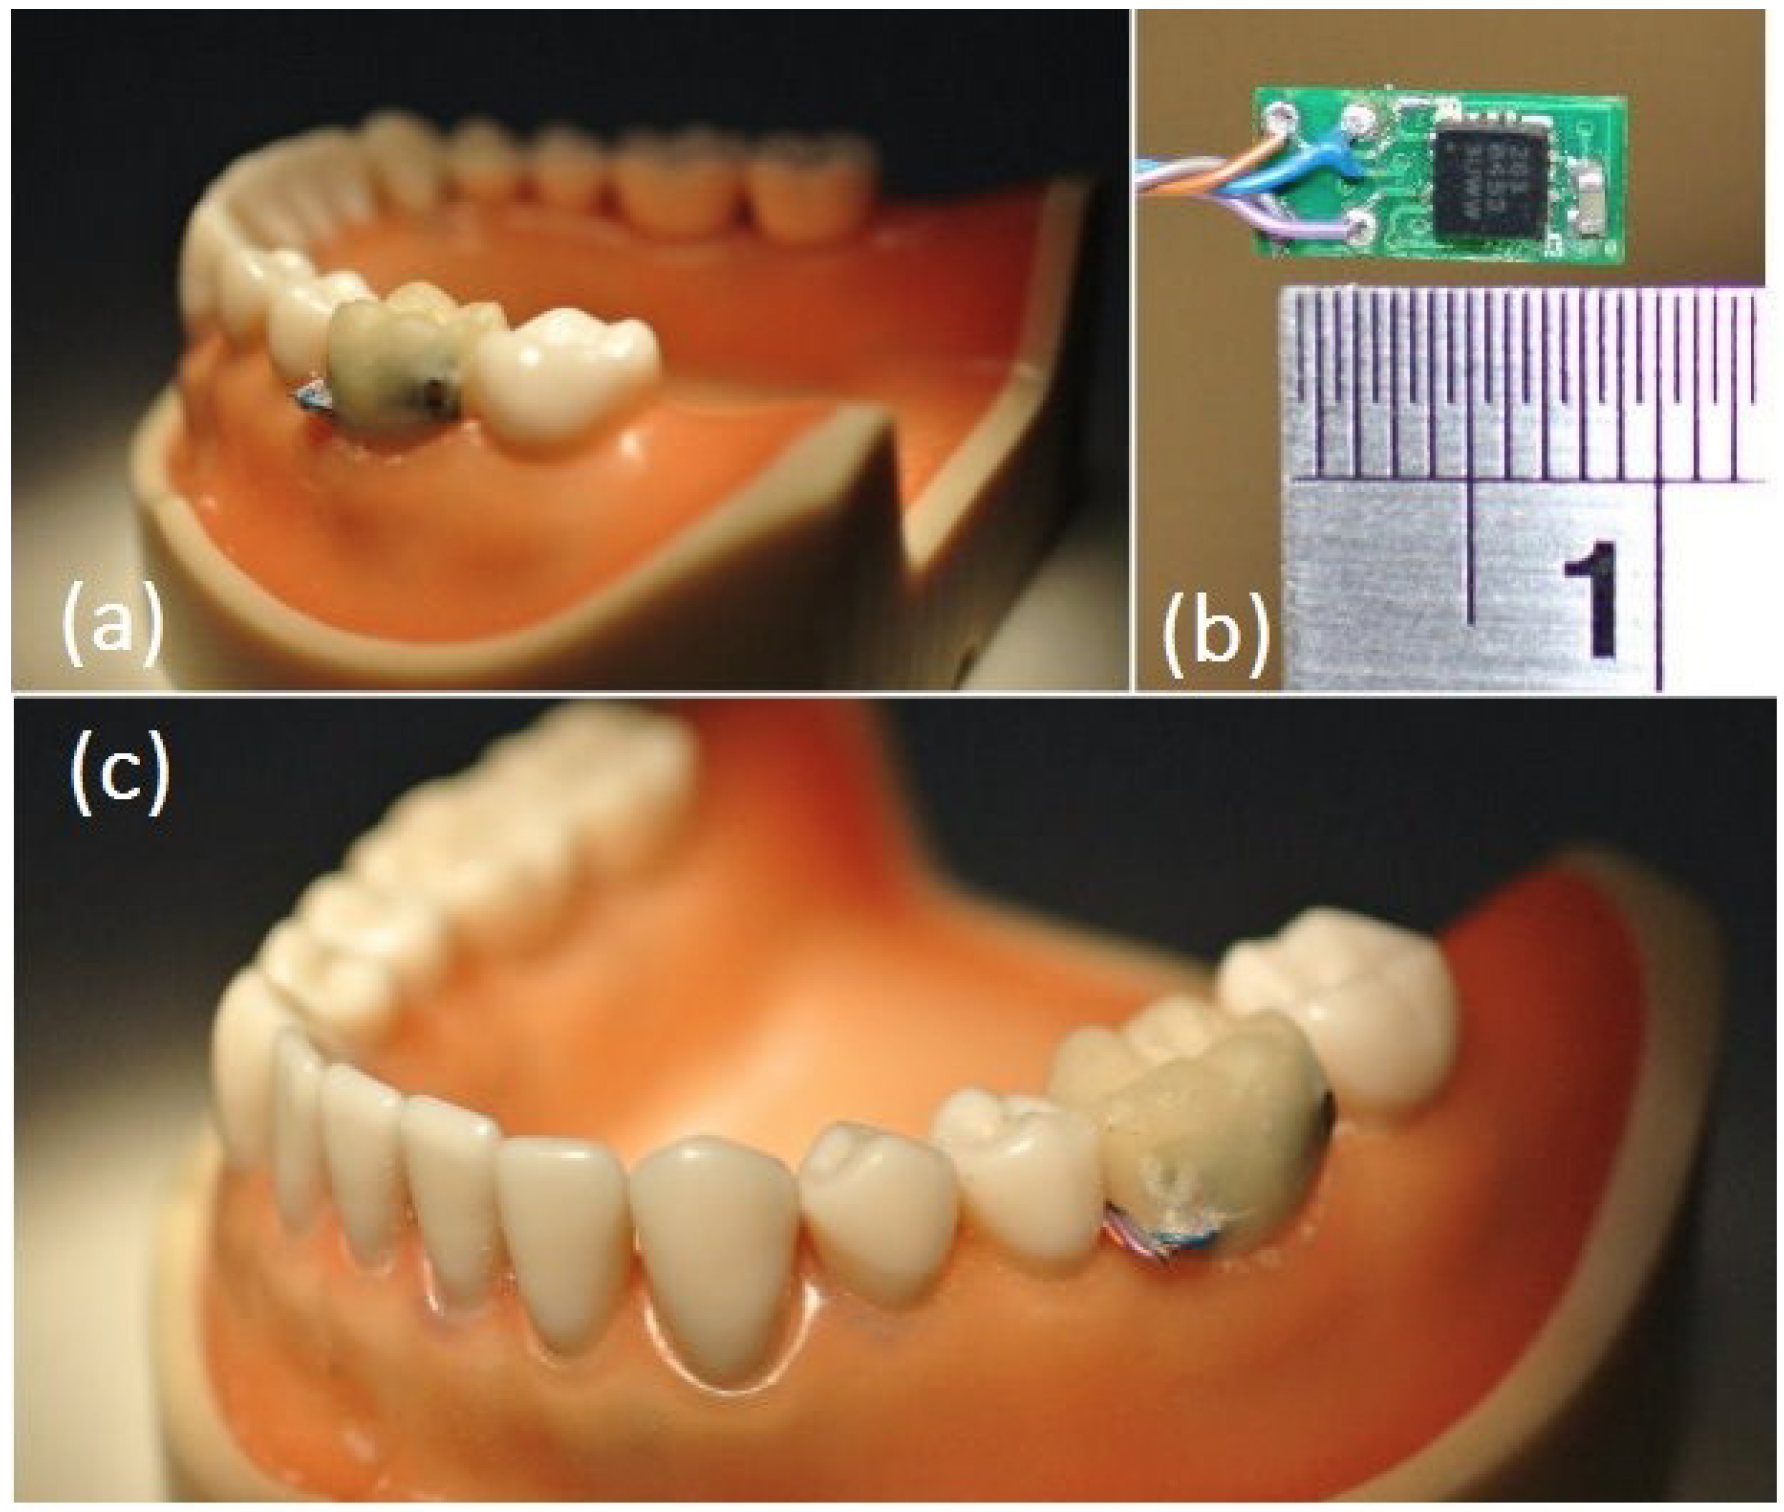
\includegraphics[width=10cm]{image/teeth}
\caption{The breakout board with (b) tri-axial accelerometer and (a)(c) sensor embedded denture.}
\label{teeth_overview}
\end{figure}

\subsection{System Overview}
The system consists of two main components: (a) an oral sensory unit; and (b) oral activity classifiers. 

\subsubsection{Oral Sensory Unit}
Figure 1(b) shows a small breakout board with a tri-axial accelerometer sized 4.5 mm x 10 mm. This small breakout board is sufficiently small to be embedded inside a removable artificial tooth, as shown in Figs. 1(a) and 1(c). To ensure that this sensor board is safe and saliva-proof for human mouth placement, we carefully coated the sensor board with dental resin. In actual system deployment, this sensor board would include a small Bluetooth radio capable of wirelessly transmitting sensor data to a nearby mobile phone for data analysis and oral activity recognition. In the current proof-of-concept system, we have yet to place a Bluetooth radio on this oral sensory unit; therefore, thin wires are used to connect the sensor board to an external data-logging device for data retrieval and power. These thin wires also protect users from accidentally swallowing the sensor units. 
Oral Activity Analysis
Oral activity recognition comprises the following three steps: (1) data preprocessing, (2) feature extraction, and (3) data classification. These steps are described as follows: 

\textit{Data preprocessing}
\newline
The sampling rate of the accelerometer sensor is set to 100 Hz. The system first divides the accelerometer data into windows of 256 samples with a 50\% overlap between consecutive windows \cite{KristofVanLaerhoven:2000}. In each data window, the system extracts the time-domain and frequency-domain features shown in Table \ref{teeth_features}. 
Because people have different mouth and teeth specifications, sensor orientation can change for different users. Thus, accelerometer readings must be adjusted and calibrated using a rotation matrix. During the calibration phase, the proposed system asks users to hold their head straight and still for a few seconds during the application of Rodrigues' rotation formula to compute this rotation matrix. Each oral sensor unit has its own rotation matrix, which is used to transform its sensor readings from the device's coordinates to real-world coordinates. This normalization procedure reduces the negative effect of errors caused by varying device orientation. Because this normalization procedure reduces, but does not completely remove this error, the system also extracts orientation-independent features based on the magnitudes of x-, y-, and z-axis acceleration. For each sample at time t, its magnitude data is calculated as $\sqrt{x_{t}^{2}+y_{t}^{2}+z_{t}^{2}}$.


The normalized (orientation-dependent) feature set and the orientation-independent feature set have different characteristics. The normalized feature set retains separate information on tri-axial acceleration values, which are required for distinguishing activities involving both vertical and horizontal movements. In contrast, the orientation-independent feature set is based on the magnitude value, in which its precision is less affected by changes in device orientation; thus, it is suitable for distinguishing activities that depend on the movement scale.

\textit{Feature extraction}
\newline
Table \ref{teeth_features} lists the time-domain and frequency-domain features extracted from each data window. Frequency-domain features are computed using the FFT algorithm. Both real and imaginary components of FFT coefficients in the 256-sample window are used to generate 256 features. Overall, the system trains activity classifiers by computing and extracting the following two feature sets: 807 features (269 features per axis acceleration) from the normalized feature set, and 269 features from the device-independent feature set.


\textit{Training Classifiers}
\newline
Our system implements three classifiers: the C4.5 Decision Three (DT), the Multivariate Logistic Regression (MLR), and the Support Vector Machine (SVM). The SVM classifier uses the radial basis function kernel and one-against-one multiclass classification, and it is further optimized by an additional parameter selection and data scaling. To filter out redundant and irrelevant features, we performed feature selection based on the correlations between features. Low-relevance features with low correlation are filtered out. We adopted principal component analysis [5] as a feature selector, in which the number of relevant features was reduced to 137. 
For each classification algorithm of the DT, the MLR, and the SVM, we trained two classifiers: person-dependent and person-independent. A person-dependent classifier uses data from all users (i.e., 8 participants in our study) to train a generalized activity model for recognizing the oral activities of different users. Conversely, a person-independent classifier uses 7 users' data to train a specify activity model for recognizing remaining person's oral activities.

\begin{table*}[!ht]
\centering
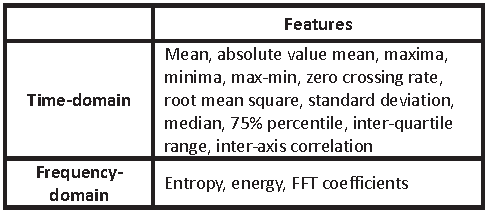
\includegraphics[width=10cm]{image/teeth_table1}
\caption{Adopted features for oral activity recognition.}
\label{teeth_features}
\end{table*}

\subsection{Experimental Evaluation}
We conducted a laboratory experiment to evaluate the accuracies of different classification algorithms.

\subsubsection{Experimental Procedure}
Eight users (5 males and 3 females) participated in this experiment. They were asked to install the oral sensor unit inside their mouth while performing each of these four oral activities: chewing, drinking, talking, and coughing. Because it was not possible to customize a removable tooth for each participant, we used dental cement to fix the sensor units to each participant's tooth. For each activity, we collected 15 samples from each participant. Each sample consisted of 2.56 seconds of a specific activity performance. For the coughing data, participants were asked to cough continuously. For drinking data, participants were asked to drink a bottle of water. For chewing data, participants were asked to chew gum or to imitate the action. For speaking data, participants were asked to read a section of an article. We collected 480 activity samples from the 8 participants performing these four oral activities. Person-dependent and person-independent classifications used the same data set collected from the experiment.

\subsubsection{Results}
We conducted 10-fold cross-validation and leave-one-person-out cross-validation to measure the accuracies of the person-dependent and person-independent classifiers. For the person-dependent classifiers, each round of cross-validation involved using all of each participant's data for both training and testing. Table \ref{teeth_pdc} shows the mean F-measure accuracy results. The SVM (93.8\%) classifier outperforms both the DT (52.2\%) and MLR (60.5\%) classifiers.  

For the person-independent classifiers, each round of cross-validation involved using 7 participants' data for training, and the remaining participant's data for testing. Table \ref{teeth_pdc} shows the mean F-measure accuracy results. Again, the SVM (59.8\%) classifier outperformed both the DT (40.8\%) and MLR (55.9\%) classifiers. Reasons for the low-accuracy result in the person-independent classifier are as follows.
First, because people's teeth and mouth structure are different, their sensor placements are also (slightly) different, thus creating variations in the motion data. Second, people perform oral activities differently; for instance, some people chew or talk faster, slower, harder, or softer. It is possible to improve the accuracy of person-independent classification by extending the training set to include different sensor placements and oral activity types.

\begin{table*}[!ht]
\centering
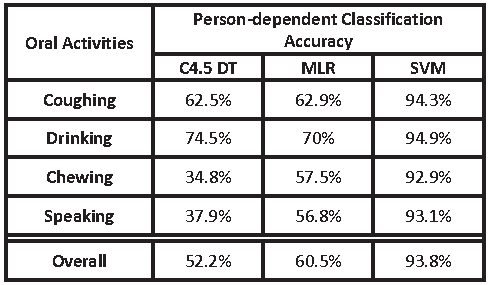
\includegraphics[width=10cm]{image/teeth_table2}
\caption{F-measure accuracy of oral activity recognition with a person-dependent classifier.}
\label{teeth_pdc}
\end{table*}

\begin{table*}[!ht]
\centering
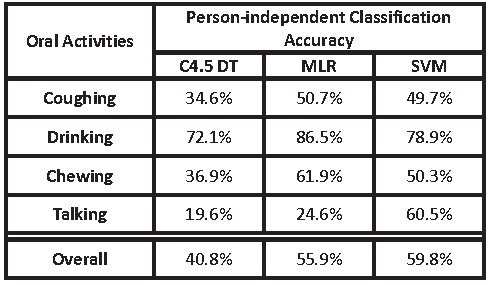
\includegraphics[width=10cm]{image/teeth_table3}
\caption{F-measure accuracy of oral activity recognition with a person-independent classifier.}
\label{teeth_pidc}
\end{table*}

\subsection{Discussion}
This is a feasibility study of an oral sensory system that detects human oral activities. We identified the following challenges for the proposed oral sensory system.
\newline
\textit{Data logging and transmission}
\newline
If an application does not require real-time monitoring, sensory data can be temporarily stored on the sensor device. When users remove their artificial teeth, for example, for disinfection and storage, small electrodes on the surface of the artificial teeth are used to connect to the sensor board and retrieve stored sensor data. For a real-time monitoring application, the sensor board must have a low-power wireless radio (e.g., Bluetooth) to transmit sensor data to a nearby smartphone for data analysis and activity recognition. Another possible data transmission medium is intra-body communication \cite{Hachisuka:2003}, which has lower power consumption compared to wireless radio communication.
\newline
\textit{Energy}
\newline
Because users must remove artificial teeth for daily disinfection and storage, we surmise that a recharging and storage station will be required, similar to that of an electric toothbrush, in which users would place the cleaned artificial teeth on this station for battery recharging and data retrieval. 
\newline
\textit{Safety}
\newline
Because of the sensor placement inside the mouth, the safety concern is paramount. All electronic components must be sealed securely and tightly. In the event that the sensor units are mistakenly swallowed, they will pass the human body without causing any harm. Its safety requirements are similar to those of capsule endoscopy, in which patients swallow a camera pill. Because our current prototype (Figure \ref{teeth_overview}) was not considered safe, we attached a safety string to the sensor unit so that participants would not be able to swallow it.

\subsection{Summary}
For this study, we designed and developed an oral sensory system that can recognize human oral activities. Our results from a laboratory experiment with 8 participants demonstrate the feasibility of this oral sensory system in recognizing the following four human oral activities: speaking, chewing, drinking, and coughing. We found that a person-dependent SVM classifier achieved a high F-measure accuracy of 93.8$\%$, whereas a person-independent SVM classifier achieved only an F-measure accuracy of 59.8$\%$. 
Because the mouth is an opening into human health, this oral sensory system has the potential to enhance exiting oral-related healthcare monitoring applications such as dietary tracking. 




\newpage
\section{Sensing Fork: Persuasive Technology to Improve Eating Behavior using a Sensor-Embedded Fork}

Parents often experience situations where verbal persuasion 
has only limited effectiveness with their children. 
A particular case is at mealtime when parents are attempting 
to instill healthy eating habits in their children. 
For example, parents often say, \textit{``Eat your green food''} 
or \textit{``Finish up your plate.''} 
Children, however, often have little or no incentive to comply with these directives. 
Is it possible to apply computing technology to make the eating behavior training experience 
more enjoyable for children? 
Several HCI (Human Computer Interaction) projects have explored 
persuasive technologies \cite{Fogg:2002} for motivating users in diverse daily activities 
such as brushing teeth, and avoiding a sedentary lifestyle \cite{Chang:2008}, \cite{Lin:2006}. 
We believe that the playful aspects of persuasive technology and interaction 
are especially applicable to children.

A well-balanced diet is an important factor in maintaining good health. 
From a broader perspective, dietary education today includes how to eat, 
how to select ingredients, and dietary culture. 
Because diet and health are closely related, dietary education 
is and will continue to be a universally important health topic. 
In many developed countries, governments have been promoting dietary education 
by providing dietary information on websites \cite{NHS_ENGLAND, US_Agriculture} and running dietary classes at schools.

In Japan, owing to concern over increasing unhealthy dietary habits, particularly in unbalanced nutrient consumption, 
the Dietary Education Basic Law was enacted in 2005. 
The goal of this legislation was to promote healthy dietary habits 
such that people could enjoy active 
and healthy lives \cite{Cabinet_JP}. 
Consequently, most kindergarten schools are required to have dietary education classes 
in which teachers encourage children to eat diverse types of food. 
However, it is difficult for many parents and children to continue learning 
and adopting such dietary activities at home because of the lack of time and knowledge. 
We believe that a new method for dietary education suited to the mealtime period is needed.

We therefore aim to provide an alternative method for motivating children 
to improve their eating behavior by enhancing a fork, a basic and simple eating utensil. 
This sensor-embedded fork, called a Sensing Fork, in conjunction with a mobile game, 
called a Hungry Panda, can facilitate dietary education activities 
for parents and children at home. 
To encourage eating a variety of food items, this system makes use of food \textit{color}, 
something children can easily identify and understand. 
By encouraging children to eat foods of different colors, 
the system teaches children about eating a balanced meal. 
This simple color-based food selection strategy is an alternative 
to more complex nutritional lessons that teach different food groups, 
their nutrition types, functions and roles. 
Given its simplicity, some nutritionists and 
physicians recommend a color-based dietary education method \cite{Blackburn:2005}, 
that we also adopted in our system. Japanese nutritionists have also proposed 
the ``Five-colored Balanced Food Hygiene,'' which is expected to be adopted 
to support children's dietary education \cite{goshoku}. 
The basic idea is to eat five food colors (RED, WHITE, YELLOW, GREEN, and BLACK) each mealtime. 
Our color-sensing approach is designed for children 
following this simple color-based dietary education strategy.

To detect the food color in contact with the fork, we embed a small color sensor 
at the tip of the Sensing Fork device (Figure \ref{system}). 
The Sensing Fork has other sensory and communication components including three electrodes, 
a motion sensor, a microcomputer, a Bluetooth radio, and a battery. 
By processing the sensory data, 
our system recognizes a child's eating behavior (eating actions and food colors). 
The sensory data is transmitted to the Hungry Panda game executed on a smartphone. 
The game is interactive and provides feedback 
to encourage children to improve their eating behavior.

\subsection{System Overview}
Embedding miniature sensors in utensils enables the detection of natural eating behaviors 
without introducing new tracking devices and without changing the normal operation and function of the eating utensil. 
To facilitate interaction with children, the Sensing Fork is designed to work with a mobile device. 
The Sensing Fork forwards the sensory data to the mobile device. 
The mobile device then processes the data to recognize the child's eating behaviors associated with the fork. 
The Hungry Panda game running on the mobile device interacts 
with the child according to the recognized eating behaviors.

%\begin{figure}[t]
%\begin{center}
%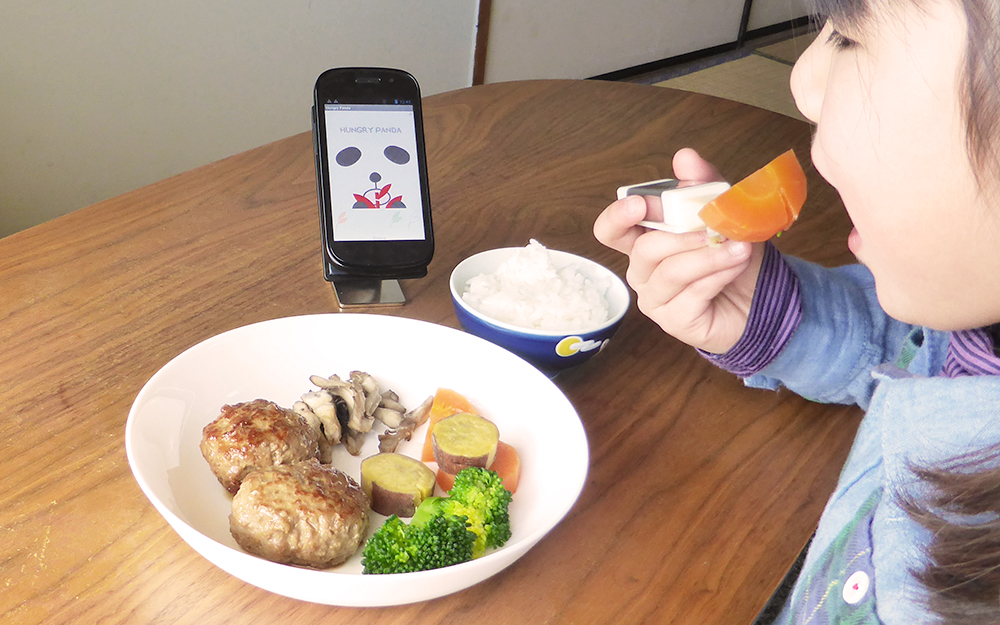
\includegraphics[width=12cm]{image/figure01-light.jpg}
%\caption{Overview of the Sensing Fork and Hungry Panda game application.}
%\label{overview}
%\end{center}
%\end{figure}

\begin{figure}[t]
\begin{center}
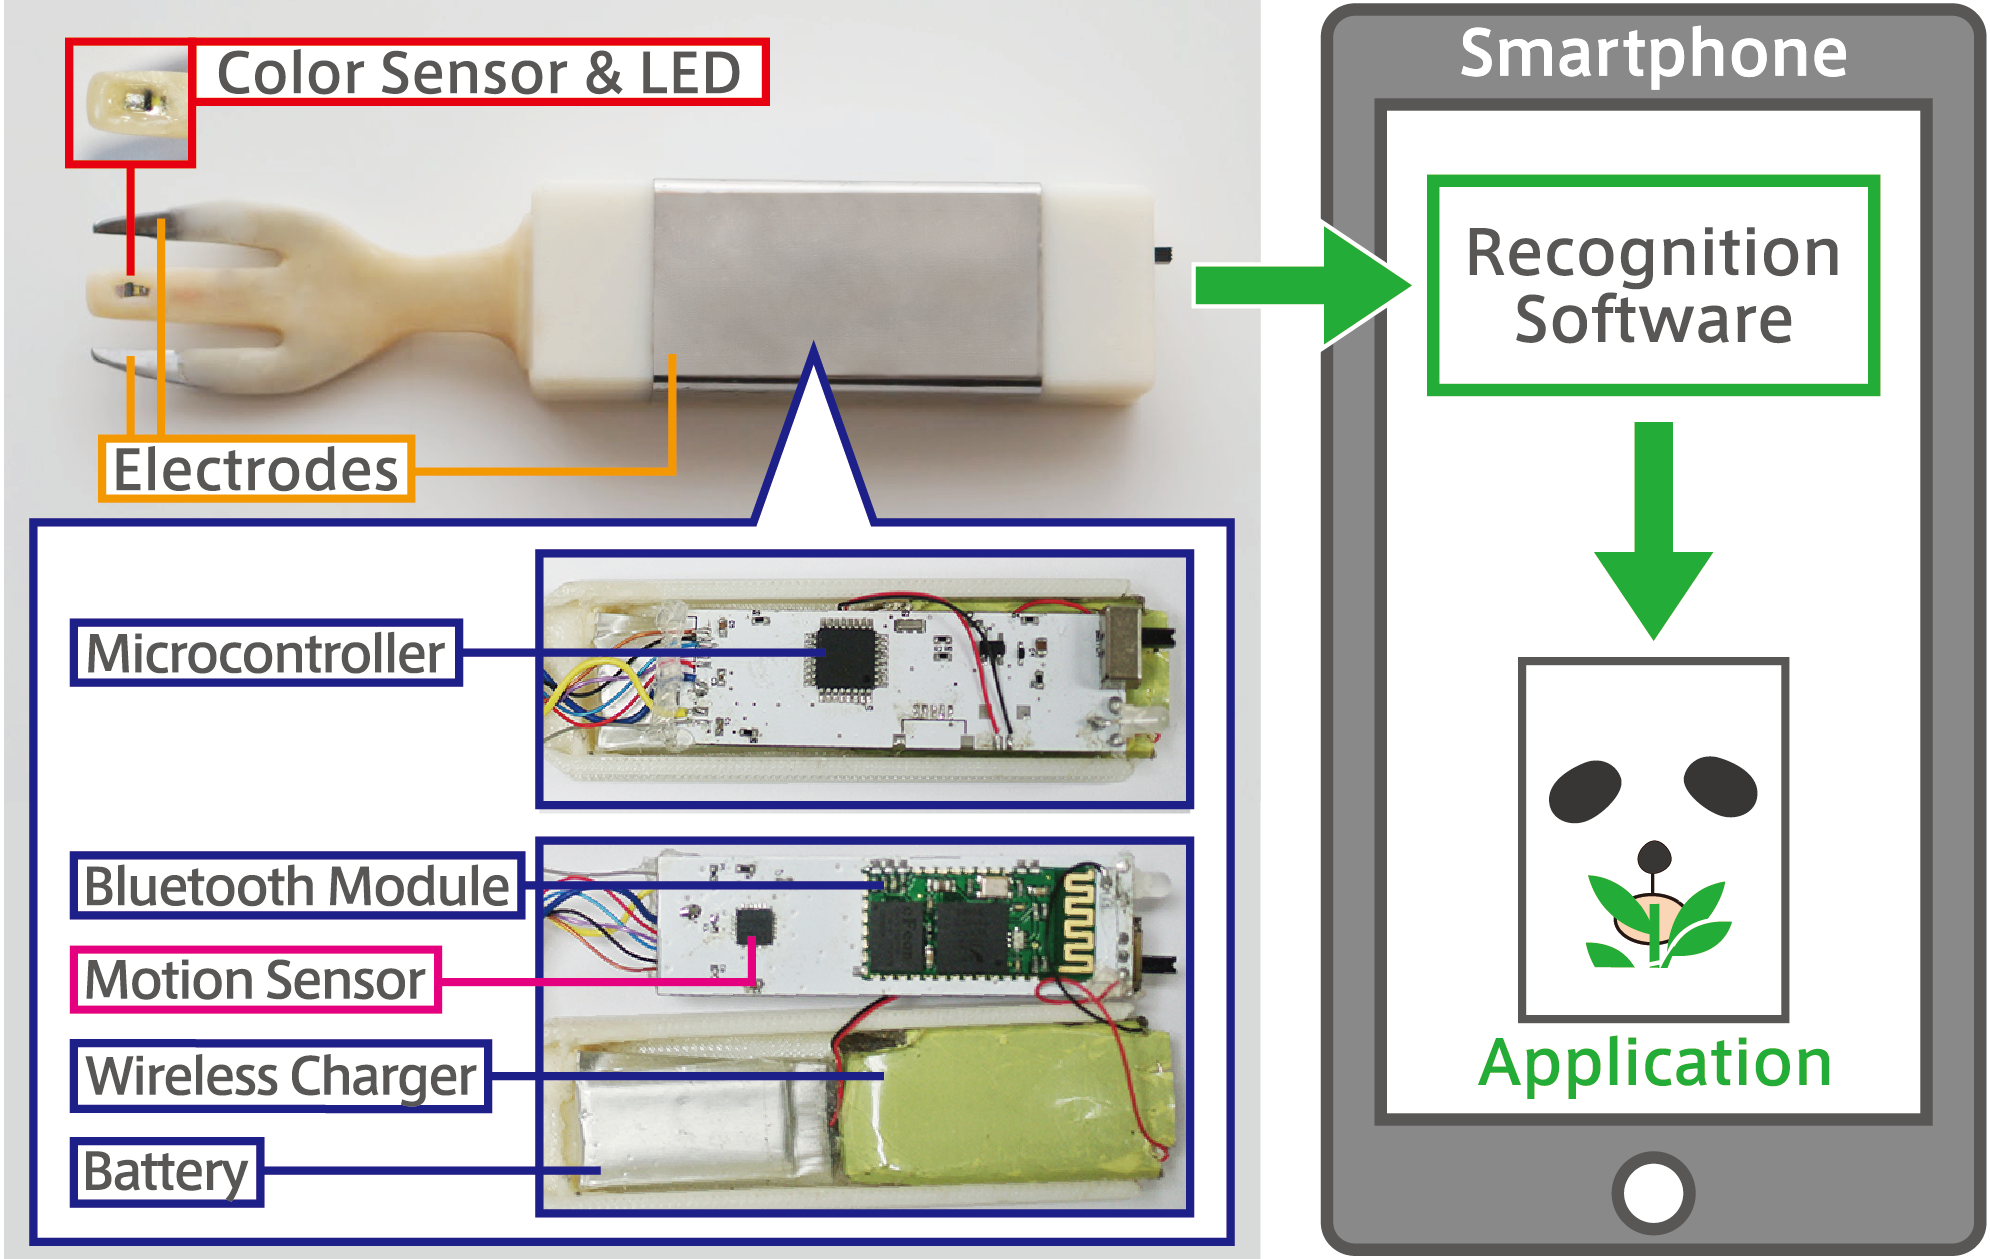
\includegraphics[width=12cm]{image/systemzu02-02.png}
\caption{System configuration. Left: The Sensing Fork prototype. Right: The software on the smartphone.}
\label{system}
\end{center}
\end{figure}

\subsection{Prototype Design: Sensing Fork}
\subsubsection{Components of the Sensing Fork}
Most of the electronic components 
are packaged and hidden inside the fork grip (Figure \ref{system}). 
The controller is an Atmel ATMEGA328P microcontroller. 
Sensor readings are collected at a rate of ten samples per second and then transmitted 
to the mobile device through a Bluetooth module. 
A rechargeable 120 mA lithium battery powers the Sensing Fork. 
There is sufficient battery power for the fork to run for two hours. 
Because it must be washed, the fork is waterproof and includes a wireless charging system. 
The fork grip is $L80 \times W25 \times H15$mm in size, 
making it easily held by small children. 

The fork's middle tine contains a tiny breakout board 
that houses a color sensor and a tiny LED light to illuminate the food contacting the fork. 
The breakout board is carefully placed between two metal tines and coated with white and transparent resin. 
The resin is dental grade, ensuring that the fork is washable and safe for eating. 

\textit{Three-electrode Conductive Probe}
\newline
Because both food and the human body are conductive, we leveraged two naive voltage dividers 
with three-electrodes to recognize two eating actions: \textbf{Poking} and \textbf{Biting}. 
As shown in Figure \ref{system} and Figure \ref{electrode}, 
two metal tines and one metal surface grip are wired to the circuit as electrodes. 
In the case of \textbf{Poking}, the measured voltage equals the supply voltage 
when the two fork's tines (electrodes) do not make contact with food. 
When the two fork tines do contact food, 
a circuit is created in which the measured voltage is altered because of the food's impedance. 
The function for recognizing \textbf{Biting} is similar. 
When a child's mouth contacts food while holding the fork's grip, i.e., the third electrode, 
it forms a circuit between the fork's grip and tine, the child's mouth, and the hand. 
The electrical current that passes through the food and child's body is low and safe. 

\textit{Six-axis Motion Sensor}
\newline
To capture human motion with the fork, the Sensing Fork includes an InvenSense MPU-6050 that integrates a three-axis accelerometer and a three-axis gyroscope into a single chip. The motion data is used to infer changes to the fork's state. 

\textit{Single-pixel RGB Color Sensor}
\newline
The single-pixel RGB 
color sensor is a TAOS TCS3414 
that outputs four-channel color readings (RGB and intensity). 
It is very small, $L2.1 \times W1.9 \times H0.9$mm. 
The color sensor samples the food color when a child pokes the food. A tiny white LED next to the color sensor illuminates the food in case the tine penetrates the food too deeply for the sensor to determine the color. 

\begin{figure}[t]
\begin{center}
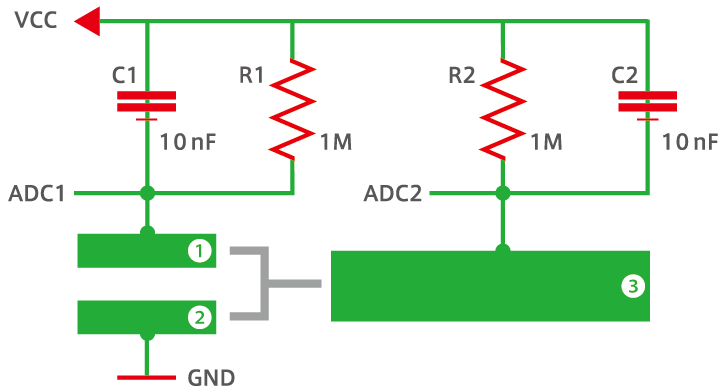
\includegraphics[width=10cm]{image/denkyoku02-02.png}
\caption{Electrodes and resistance sensing schematic. Marker 1 and 2 represent two fork's tines. Marker 3 is the fork's grip.}
\label{electrode}
\end{center}
\end{figure}

\begin{figure}[t]
\begin{center}
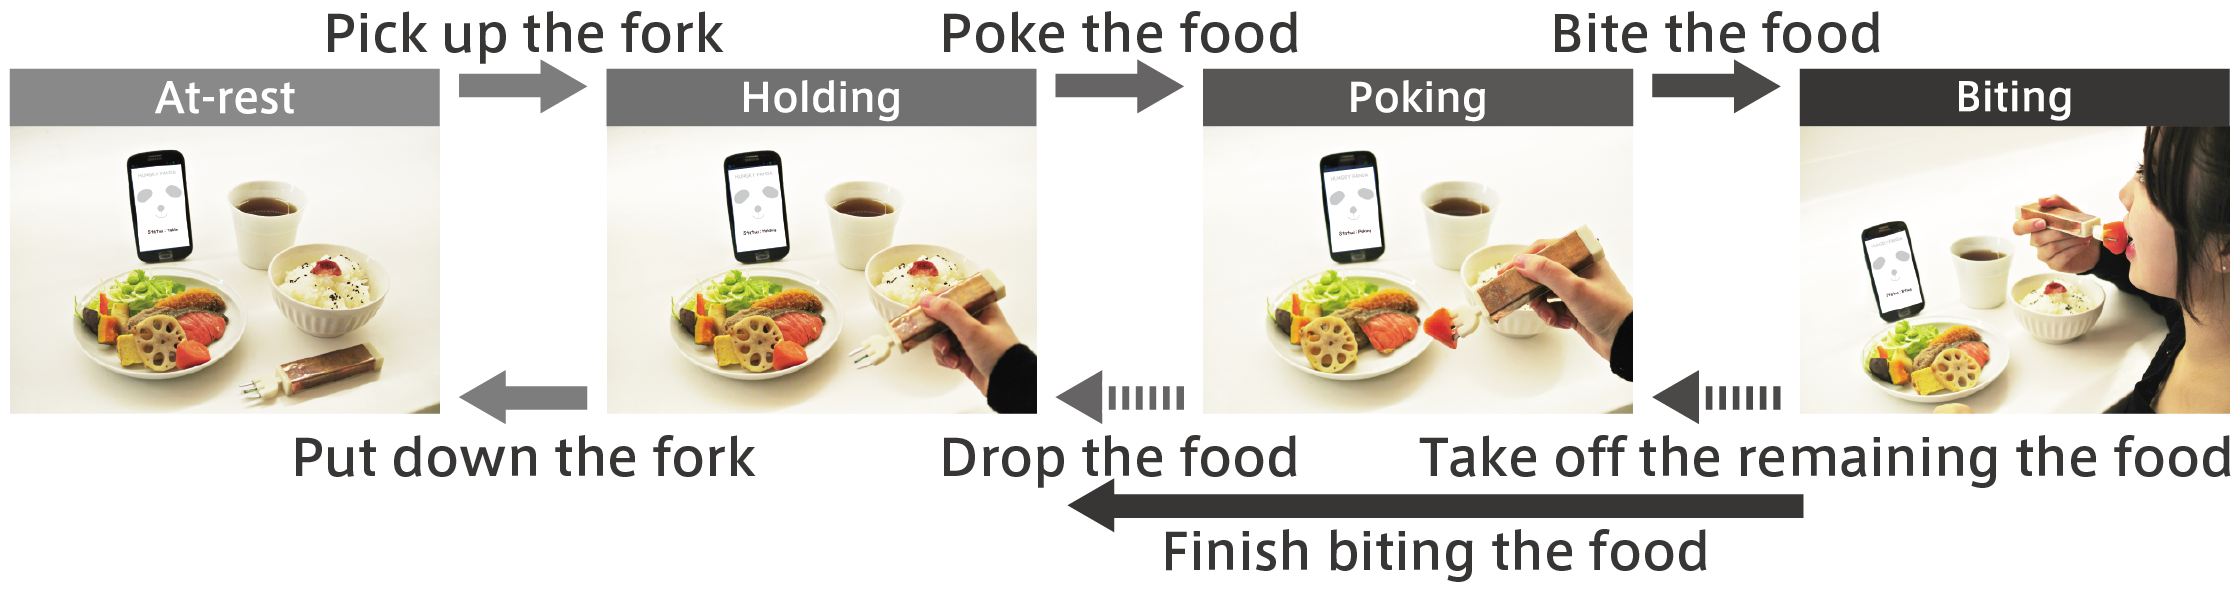
\includegraphics[width=15cm]{image/status02-02.png}
\caption{State transition diagram of eating actions.}
\label{action}
\end{center}
\end{figure}

\subsubsection{Detecting Eating Actions}
The eating action detector analyzes the sensor readings 
from the fork and determines the state of the fork during a child's eating action. 
Figure \ref{action} presents the fork's four states 
and describes the method used by the proposed system to distinguish between them. 

\textit{At-Rest}
\newline
The fork is \textbf{At-Rest} state when it is not being held by a hand. 
If the fork is the only eating utensil, this state suggests that the user is not engaging in any eating action. 
The system is able to infer the \textbf{At-Rest} state given that the accelerometer and gyroscope sensors report no motion.

\textit{Holding}
\newline
The fork is in the \textbf{Holding} state when it is being held by the hand without any food on the fork. 
This state suggests that the user has lifted the fork and may be deciding what food item to grab with the fork. 
The system infers this \textbf{Holding} state based on the presence of motion from the accelerometer and gyroscope sensors.

\textit{Poking}
\newline
The fork is in the \textbf{Poking} state 
when it is being used to poke a food item. 
The fork's tines contact the food. 
This state suggests that the user is in the process of selecting food, 
but has not inserted it into his/her mouth. 
The system infers the \textbf{Poking} state from two sensor inputs: 
(1) two-electrode tines measure a non-zero resistance value indicating the presence of food; 
and (2) the photocell sensor detects food colors. Touching food with the fork triggers the food color recognizer. 

\textit{Biting}
\newline
The fork is in the \textbf{Biting} state when the fork or food on the fork contacts the mouth. 
This state suggests that the user is biting or tasting the food on the fork. 
The system infers the \textbf{Biting} state by measuring an altered reading 
from the fork circuit connecting the child's hand, fork, and mouth. 

\subsubsection{Classifying Food Types}
Our system uses the food's color as the feature to classify the type of food that contacts the fork. 
Food type classification includes the following four functions:
(1) sample selection, (2) extracting feature, (3) training classifier, and (4) online testing. 

\textit{Sample Selection}
\newline
Because the fork's sampling rate (10 Hz) is higher 
than in human's eating actions, 
our system observes a window of sensor data for each eating action. 
Consider the case where a child is deciding what to eat next. 
The child might start by touching one food item before moving on to another, and then another. 
This can continue until the child sticks the fork tine inside a target food item. 
Thus, the sensor readings will vary initially and then stabilize when the fork penetrates a food item. 
To determine this stable window, 
our system uses a sliding window with a length of five samples and then computes a variance value for this window. 
If the variance value is lower than the threshold value, 
our system uses the sensor data in this window for inferring the food type. 
Note that the fork must also be in the \textbf{Poking} or \textbf{Biting} state. 

\textit{Extracting Feature}
\newline
Four color readings and one resistance value 
in the sample are used for classifying the food types. 
The raw color readings can vary between each poking of the same food item. 
The RGB readings increase linearly with light intensity. 
Since the ambient lighting may affect the RGB sensory readings, 
we calculate two-dimensional chromaticity values \cite{Broadbent:2004} using the RGB readings 
as features to mitigate the effect from ambient luminance. 
Note that chromaticity represents the quality of a color regardless of its luminance. 
Our system also computes the difference between the RGB values and clear readings 
as features to train a food detection classifier. 
When a child is poking a food item, the attached LED on the fork tine becomes the primary light source 
to illuminate the food's interior color. 
Based on our experiment, the fork's LED is primary in detecting food color, 
whereas the ambient light has only a limited effect. 

\begin{figure*}[!t]
\begin{center}
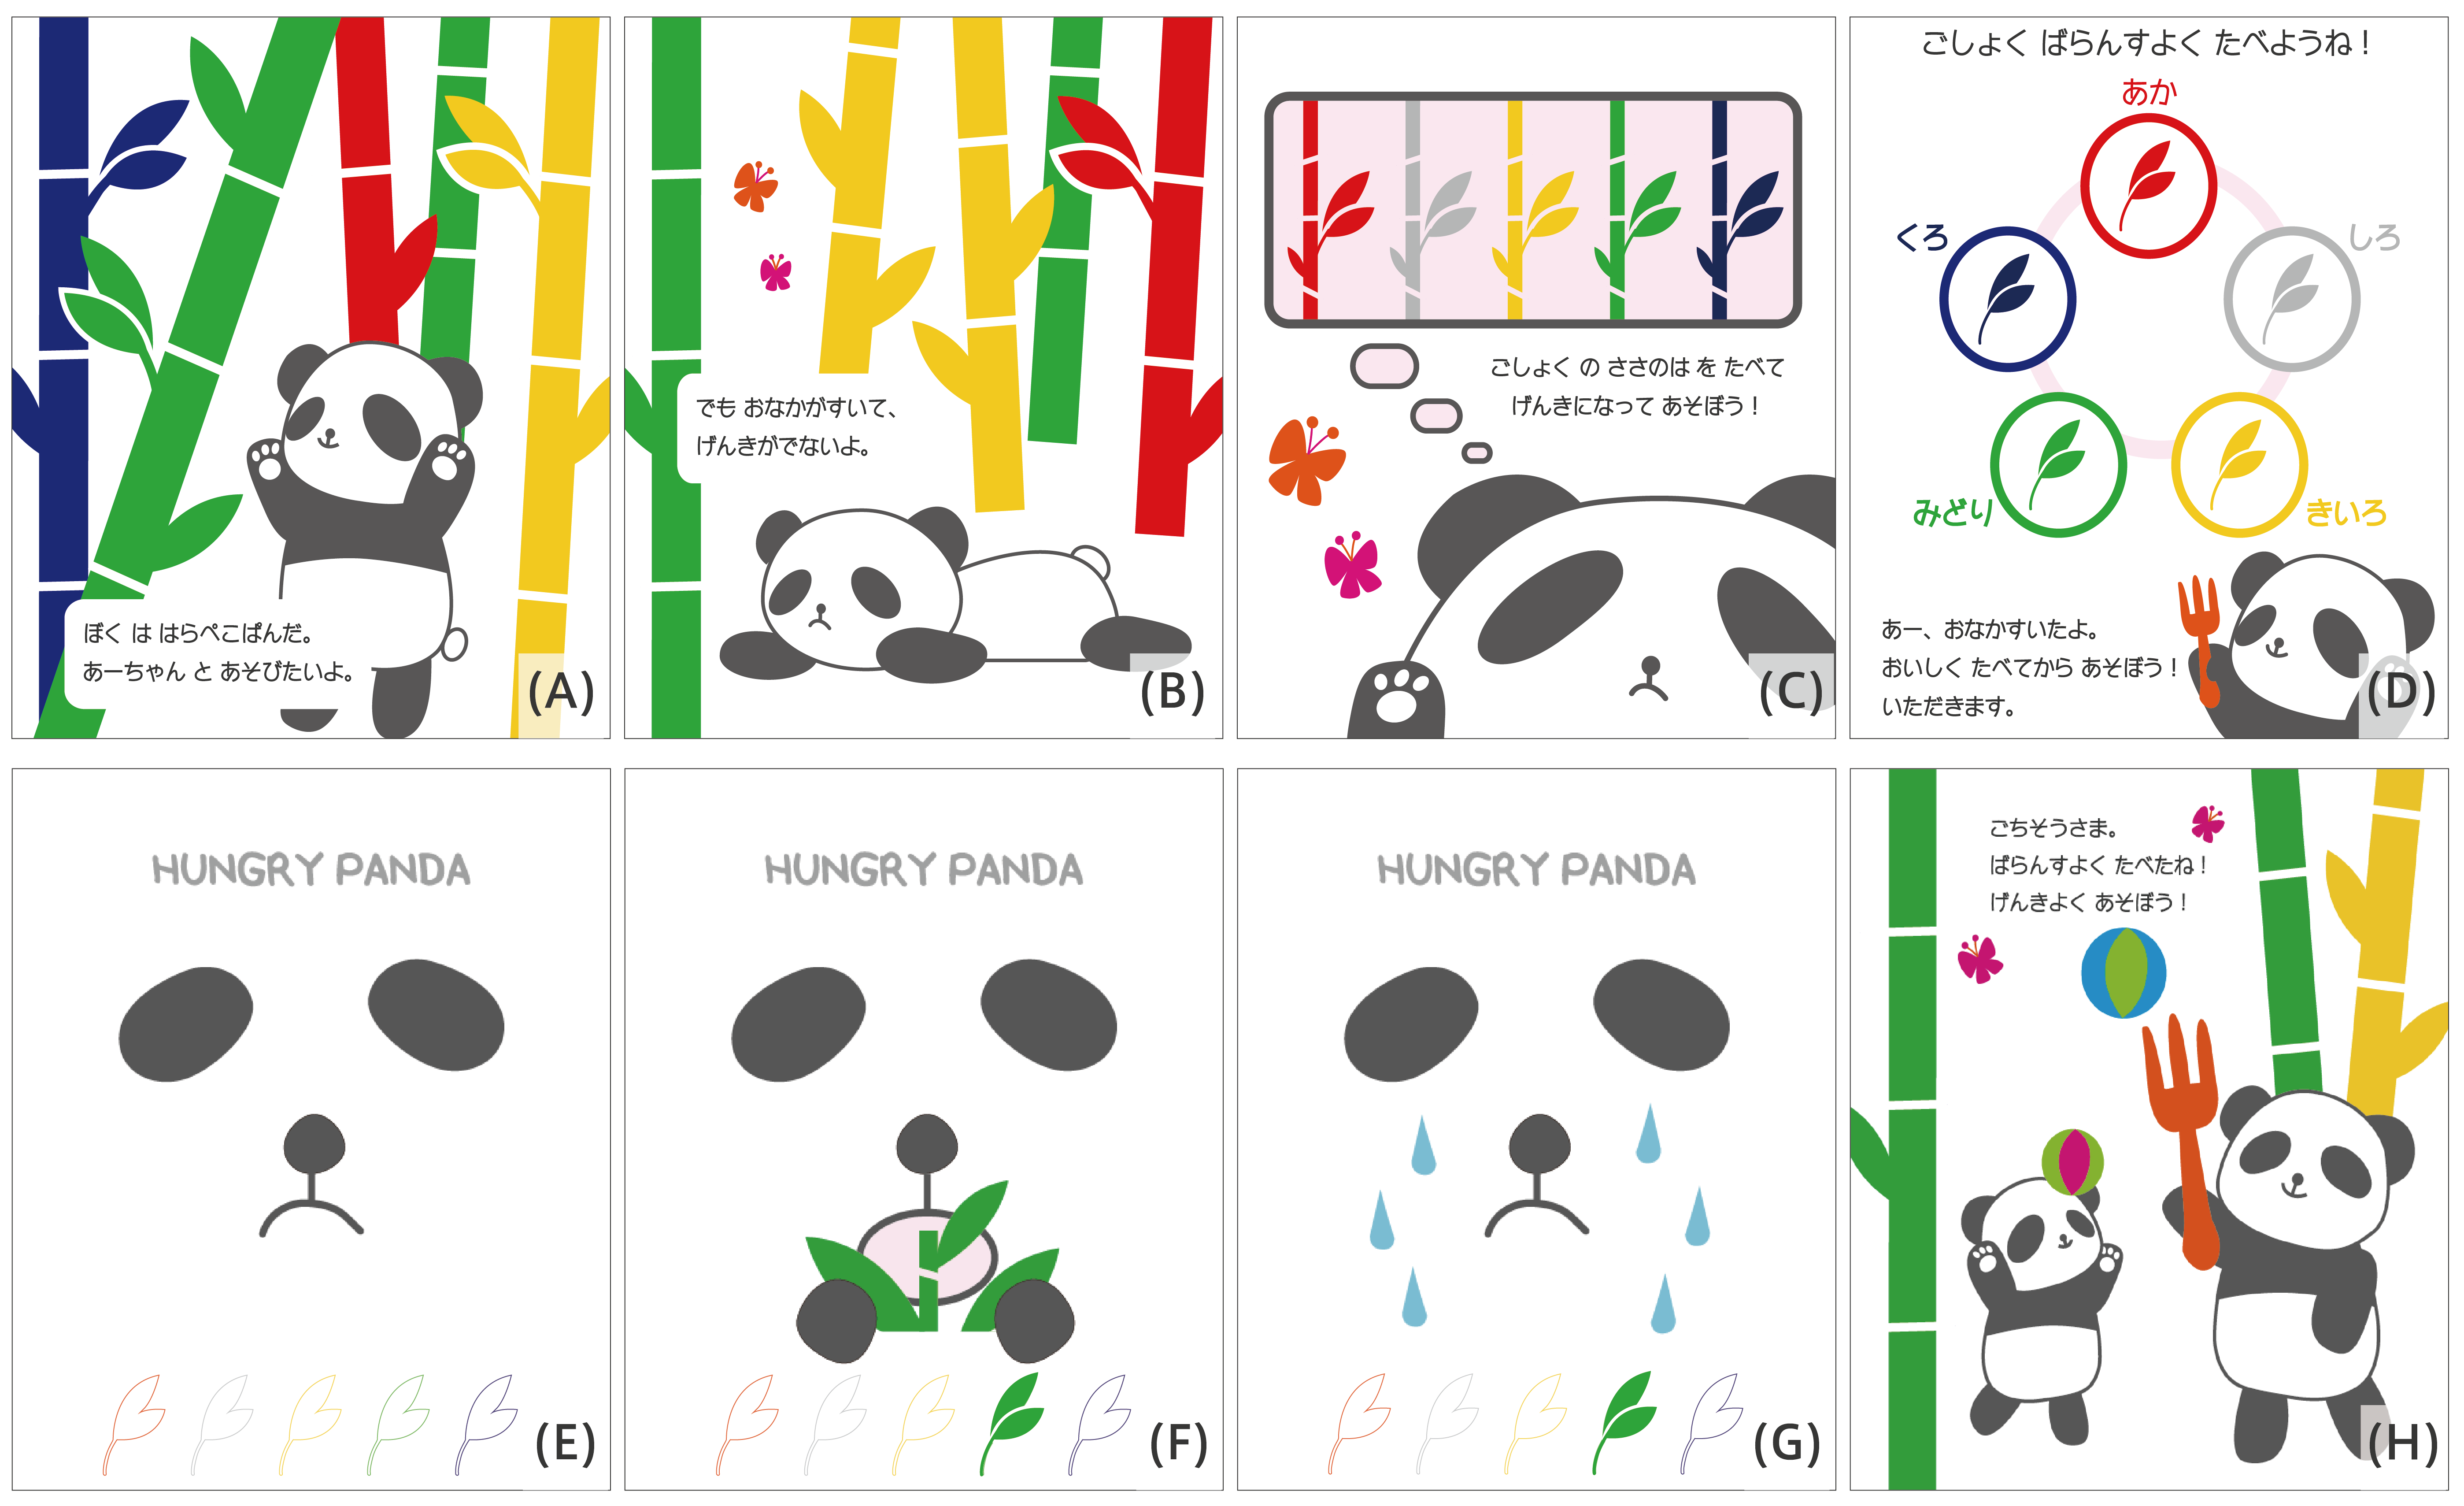
\includegraphics[width=15cm]{image/HP_app.png}
\caption{The story and flow of Hungry Panda game application.}
\label{panda}
\end{center}
\end{figure*}

\textit{Training Classifier}
\newline
A Support Vector Machine (SVM) algorithm is used to train the classifier. 
The classifier is implemented with LibSVM \cite{Chang:2011}. 
The SVM classifier uses the polynomial kernel and one-against-one multiclass classification.

The method used to train the classifier results in differing food classification performance. 
As the number of food types increases, the performance of the classifier decreases. 
This is because foods may have similar colors that are ambiguous to the classifier. 
The classifier can be trained either right before the meal or in pre-training. 
Training right before the meal (per-meal training) requires the user to collect samples before the meal is about to start. 
This determines the significant differences between ingredients that are of the same type though not identical. 
Identical ingredients may still have a slight difference in color. Cooking-style might also change the food's color. 
A pre-trained classifier is trained prior to any system deployment with food samples 
that are commonly eaten by children in the community. 
By comparison, a per-meal classifier is trained with food samples collected from a meal immediately prior to consumption. 
The advantage to using a pre-trained classifier is that it saves the user from needing to train the classifier. 
The advantage to using a per-meal classifier is accuracy, 
because the training samples are identical to the testing samples 
and because every family serves different food or at least prepares the same food differently, 
i.e., the same food but with a slightly different color. 
In other words, the per-meal and pre-trained classifier form a tradeoff between accuracy and convenience in real-life use. 

\textit{Online Testing}
\newline
In our application, the system tests five consecutive samples determined by sample selection. 
The classifier tests each sample separately. 
The system reports the results according to the most occurrences of the tested results from the five selected samples. 
Real-time classification on the Android platform was implemented using the LibSVM library for JAVA. 
Our application is able to perform online testing smoothly using an Android phone.

Our application classified the food items into five color categories (RED, WHITE, YELLOW, GREEN, 
and BLACK) according to the ``Five-colored Balanced Food Hygiene'' \cite{goshoku}. 

\subsection{Persuasive Game Application: Hungry Panda}
In this study, we focus on improving a child's dietary behavior, 
particularly by eating diverse foods with different colors. 
We developed a persuasive game application, 
called a Hungry Panda, on a smartphone to be used together with the Sensing Fork. 
The basic design for the Hungry Panda game has a digital panda imitating the child's eating behavior, 
including the eating actions and selected food colors. 
The rationale for designing it this way is to build rapport and foster sympathy for the panda, 
so that the child wants to help the panda. 
Because the panda imitates the child's eating behavior, 
the child is presented with an opportunity and a choice to help the panda 
by improving his/her own eating behavior. 
The use of a smartphone is a convenient computing and display device for many people in Japan 
and elsewhere. 
We use the panda as a virtual pet, because the panda is familiar to children 
in most Asian countries. 
The Hungry Panda game consists of two parts: 
(1) an interactive picture book for dietary education prior to eating, and 
(2) an interactive and persuasive game application for collecting points during a meal. 

\subsubsection{Picture Book for Dietary Education}
It is common for parents to read picture books aloud to their children. 
Such activities are not only important for educating children 
but also serve to foster good parent-child relationships. 
Therefore, we designed a short and simple picture book to teach color-based dietary education. 
Reading this picture book before a meal helps both parents and children to become familiar with the color-based food game. 

The game's first screen is shown in Figure \ref{panda} (A), with a panda greeting the child: 
\textit{``Hello, (the child's name). I am Hungry Panda. I want to play with you.''} 
This panda greeting is an attempt to initiate friendship with the child 
and encourage the child's sympathy for the panda. 
Figure \ref{panda} (B) is the second screen that shows a tumbled Hungry Panda: 
\textit{``However, I do not feel perky because I am very hungry.''} 
This screen gives a subconscious hint to the child that mealtime is about to begin. 
Figure \ref{panda} (C) presents the third screen: 
\textit{``Let's eat five different colored bamboos to become cheerful.''} 
This sets the goal for a properly balanced diet of different food color. 
Figure \ref{panda} (D) shows the next screen 
\textit{``Let's play after the meal. Itadakimasu (Japanese expression of gratitude before meals).''} 
This screen also provides a detailed explanation about the five-colored food items. 
This short and simple picture book encourages both children and parents 
to engage in a process that is both fun and entertaining. 
Because we encourage parents to read the picture book aloud to their children, 
we removed any vocal narration from the picture book and retain only the background sound effects. 

\subsubsection{Interactive and Persuasive Game Application}
After the picture book introduction, 
the unhappy panda appears on the smartphone screen and says, 
\textit{``I am very hungry. I want to eat''} (Figure \ref{panda} (E)). 
The panda imitates the child's eating actions, 
for instance by \textbf{Holding} or \textbf{Biting}, 
and eats the bamboo grass whose color matches the child's consumed food item (Figure \ref{panda} (F)). 
All consumed food items correspond to the five colors.

This game application specifically targets 
two common eating problems\footnote{Statistical Surveys conducted by Ministry of Health, 
\newline Labour and Welfare of Japan in 2005. 
\newline http://www.mhlw.go.jp/toukei/list/83-1.html}. 
\textbf{Picky Eating}: 
The score (expressed as bamboo grass points and displayed at the bottom of the screen) improves 
when the user eats food with a different colors. 
This encourages the child to continue eating to collect more points. 
At the same time, the child is helping to feed the Hungry Panda. 
\textbf{Distraction}: 
The system generates various sounds as an alert to the child. 
For example, when the child stops eating or 
puts down the Sensing Fork for a certain time period, 
the panda cries and exclaims \textit{``want to eat more''} (Figure \ref{panda} (G)). 
When the child picks up the Sensing Fork again, the panda laughs. 
In the game design, holding the Sensing Fork is not only a way for the child 
to show an interest in helping, 
it also encourages the child to concentrate on eating, thereby avoiding distractions. 
Pressing the finish button produces an animated reward for the child's good behavior 
---the higher the points obtained, the more impressive the animation (Figure \ref{panda} (H)). 

\subsection{Experimental Evaluation}
We conducted two types of experimental evaluation on the Sensing Fork using a smartphone. 
This section describes the results for detecting eating actions and classifying food colors. 

\begin{table}[t]
\begin{center}
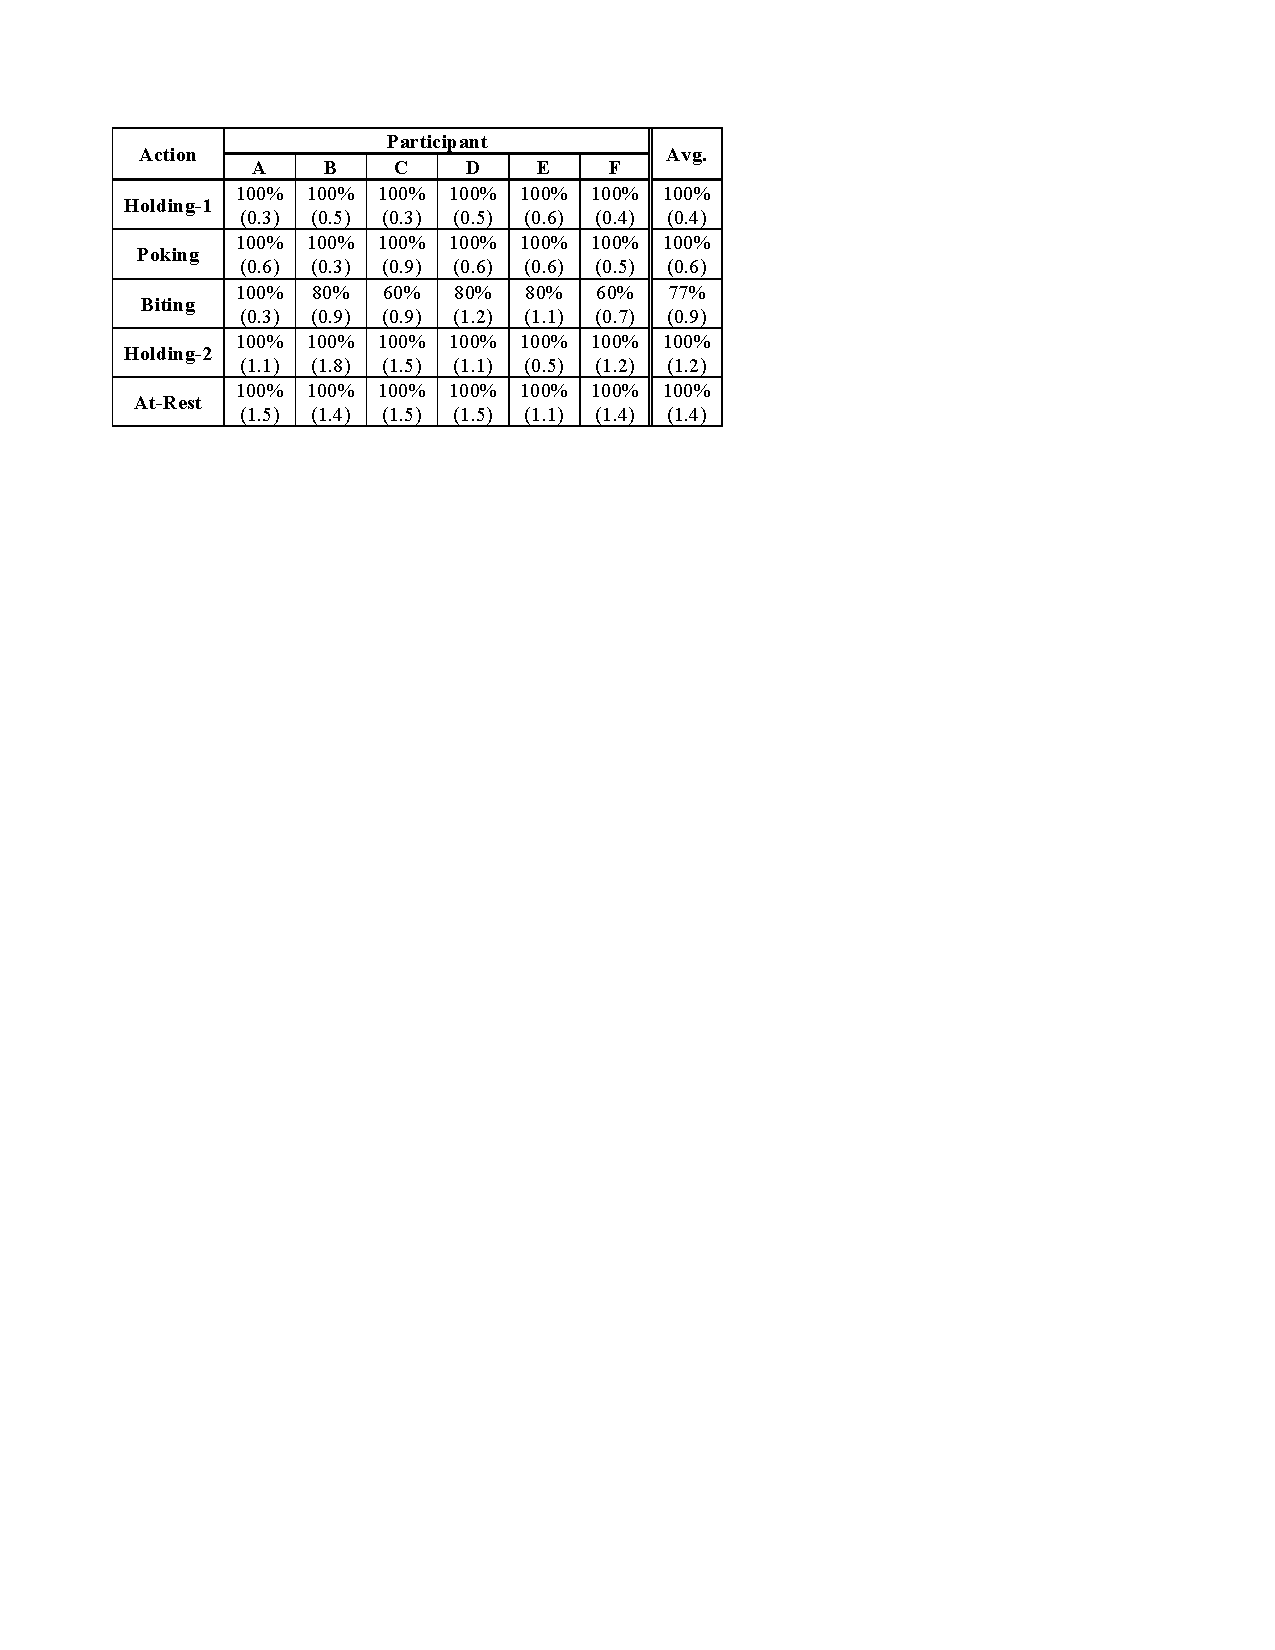
\includegraphics[width=12cm]{image/tables01.pdf}
\caption{The accuracy of detecting each eating action. The numbers in parentheses denote the average time (sec.) required to detect each eating action.}
\label{table1}
\end{center}
\end{table}

\begin{table*}[t]
\centering
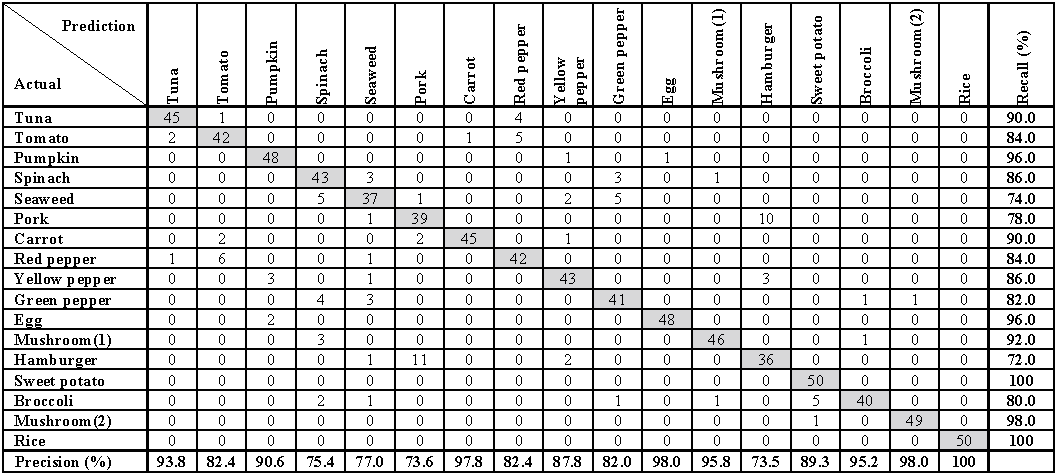
\includegraphics[width=15cm]{image/table2.ps}
\caption{The confusion matrix of classifying food types. (1)Shiitake Mushroom.  (2) Eryngii Mushroom.}
\label{table2}
\end{table*}

\subsubsection{Results for Detecting Eating Actions}
To confirm the ability to detect eating actions, 
we recruited six participants (three men and women, aged 21-28) 
and asked them to eat a certain food item, i.e., a bite-size cube of cheese, five times. 
We instructed each participant to put the Sensing Fork back on the table 
to examine the recognition accuracy for the completion of a single sequence in eating actions. 
Each eating sequence included \textbf{Holding-1}, 
\textbf{Poking}, \textbf{Biting}, \textbf{Holding-2}, and \textbf{At-Rest}, in that order. 
\textbf{Holding-2} was the time when the fork left the participant's mouth. 
Each participant repeated the above eating sequence five times. 
All participants were using the Sensing Fork for the first time. 
We did not describe the system to them in advance.

Table \ref{table1} shows the accuracy of eating action detection and the average time required for detection. 
%the number of times each eating action was detected and the average time required for detection. 
The overall recognition rate was 95\%. 
However, the \textbf{Biting} recognition rate was only 77\%. 
\textbf{Biting} was falsely detected as \textbf{Holding-2}. 
On observing the falsely recognized \textbf{Biting} action on the video, 
we noticed that the average time taken was only 0.1s, 
whereas a correctly recognized \textbf{Biting} lasted around 0.9s. 
Thus, when the fork touched the participant's mouth for only a brief moment, it was incorrectly recognized. 
This problem stems from the limitation in the implementation that set the recognition interval as 0.1s. 
This interval was set low in order to conserve battery power. 
We believe that the recognition rate will be much improved by modifying the interval. 

As shown in Table \ref{table1}, 
the average time for detecting the eating state was 0.9s. 
Notably, however, detecting \textbf{At-Rest} required 1.4s. 
This is because the fork infers it is \textbf{At-Rest} 
when it remains motionless for more than one second.
However, in general, actions such as putting down 
and lifting the fork cannot be repeated at high speeds and therefore 
this is not considered a problem. 
Further, \textbf{Holding-2} required an average of 1.2s. 
This resulted from a problem with the experimental program. 
Specifically, a sample animation of around 2.0s was displayed after the \textbf{Biting} action 
and the state did not update until the end of the animation. 
The actual detection time is thought to be equivalent to \textbf{Holding-1}. 

\begin{figure}[t]
\begin{center}
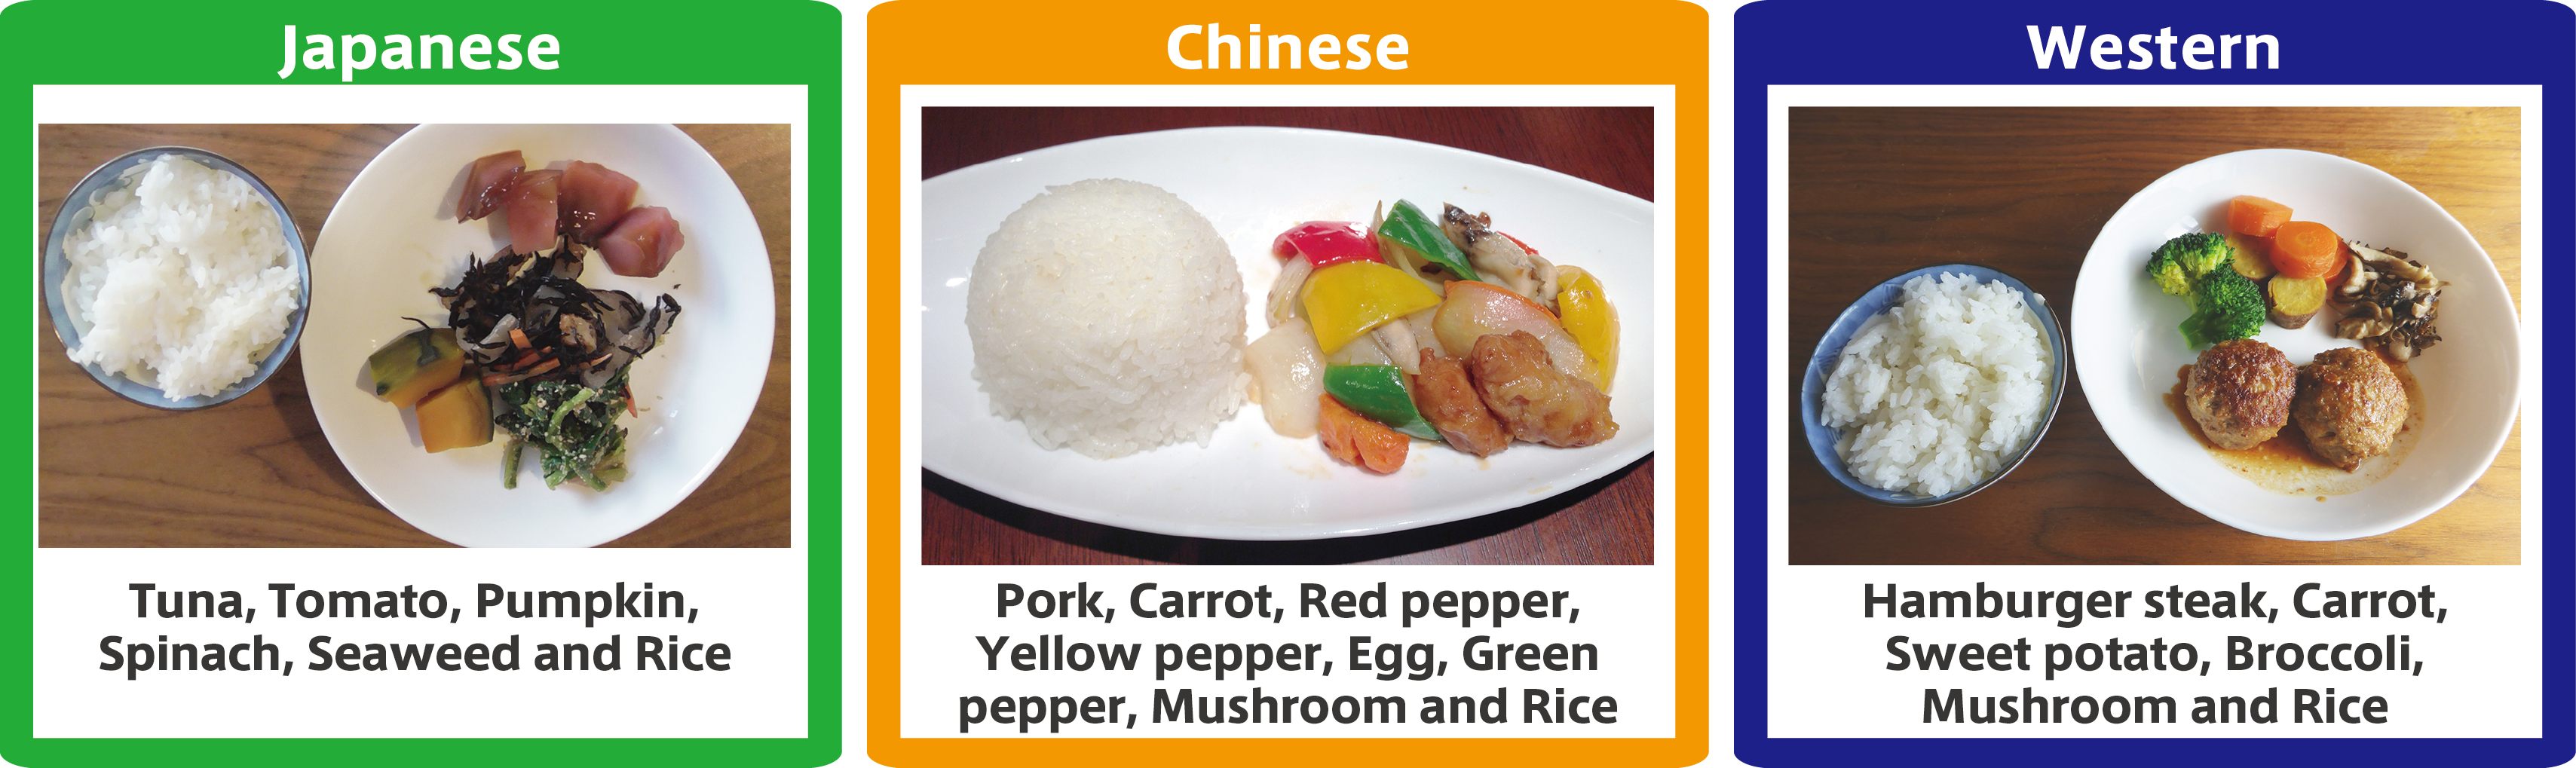
\includegraphics[width=14cm]{image/recipe01-01.png}
\caption{The examples of food items in three cuisines.}
\label{recipe}
\end{center}
\end{figure}

\subsubsection{Results of Classifying Food Types}
To examine the accuracy in classifying the food types, 
we collected food items from three different cuisines: 
Japanese, Chinese, and Western cuisines typical in Japanese households (Figure \ref{recipe}). 
%Each cuisine cuisines included multiple food types providing a balanced diet. 
Each cuisine included multiple food types providing a balanced diet.

We collected food samples using the Sensing Fork to perform a poking action with the food item. 
Based on the three different cuisines, 
we collected 17 types of food items and 50 samples of each, 
because the color of the same ingredient could change with the cooking method. 
In each experiment, we poked the food item ten times. 
The collected dataset contained 850 samples from the 17 food types. 
We conducted a 10-fold cross-validation to evaluate the F-measure accuracy of the food-color classifier. 
Each round of cross-validation randomly divided all the samples into a training set and testing set. 
The overall F-measure accuracy was 87.5\% in this experiment. 
Table \ref{table2} shows the confusion matrix for the result 
that evaluated classifying 17 food types under the cross-validation. 
Improper poking caused a few incorrect classifications. 
Most incorrect classifications were caused by foods with similar colors from the sensor's viewpoint. 
For example, pork and hamburger steak, yellow pepper and pumpkin, tuna and red pepper, 
and carrot and tomato were similar groupings. 
We further classified the 17 food types into three categories 
---Japanese, Chinese, and Western--- 
and evaluated their F-measure accuracy individually. 
Because individual cuisine has less ambiguous food types, 
the accuracies of the Japanese, Chinese, 
and Western cuisines were 94.7\%, 96.2\%, and 93.8\%, respectively. 
Samples from the three cuisines were also used in our user study with the children. 
The food samples were not only used to evaluate the performance of the Sensing Fork 
but also to train the classifiers used in the Hungry Panda game during the user study. 

%\subsection{User Study}
%We conducted a real-life user study involving five mother-child pairs 
%who tested the Sensing Fork and Hungry Panda game at home. 
%This study assessed how effective our system performed in residential settings. 
%This study also evaluated how effective our system addressed children's picky eating 
%and distraction problems 
%and the effectiveness of the system's dietary education for the mother-child pairs. 
%
%\subsubsection{Procedure}
%Table \ref{table3} shows the profiles of the five mother-child pairs, 
%including the age/gender of each child, the child's eating problem, 
%and the child's disliked foods as reported by the child's mother. 
%All participants were Japanese, living in Japan. 
%We denote each child as Child-A, ..., Child-E and 
%each mother as Mother-A, ..., Mother-E. 
%Child-A and Child-D are siblings. 
%That is, the mother of Child-D is also Mother-A. 
%All the children used our system for the first time 
%and did not receive official instructions for the system. 
%We did explain the procedure for the user study 
%and provided a user study set to the mothers directly. 
%The user study set contained a Sensing Fork with a wireless charger, 
%a smartphone with a charger, a diary, and the basic instruction booklet. 
%
%The user study consisted of two parts: 
%a nine-day real-life user study and a post-meal survey. 
%In the user study, we asked each mother to take pictures 
%of the dinner plates before and after meals, to take videos during mealtime, 
%and to note comments and impressions in a diary after eating. 
%To determine what effect our system has on eating habits, 
%the children used our system on days 4-6 (Term 2) 
%and used a regular fork on days 1-3 (Term 1) and 7-9 (Term 3). 
%We also asked the mothers to make three kinds of meals 
%according to the cuisines used in the experimental evaluation: Japanese, Chinese, and Western. 
%We specified the main dish (sashimi tuna, sweet-and-sour pork, and hamburger steak) 
%and asked them to include five colored food items (RED, WHITE, YELLOW, GREEN, and BLACK) 
%as well as foods that the child dislikes. 
%To compare the eating behavior of each participant during the different terms fairly, 
%participants repeated each cuisine three times. 
%For example, participants would eat Japanese on the 1st, 4th, and 7th day, 
%Chinese on the 2nd, 5th, and 8th day, and Western on the 3rd, 6th, and 9th day. 
%The cooking-style and ingredient selection were not strictly managed. 
%For instance, some mothers put tomato sauce 
%and others put demi-glace sauce on their hamburger steaks. 
%To avoid the disturbing the dining atmosphere, 
%we were physically absent during the user study. 
%A camera was setup to record videos of all meal sessions. 
%In the post-meal survey, we asked the mothers to complete a questionnaire 
%and participate in a one-hour oral interview. 
%The questions and results of the questionnaire are summarized in Table \ref{table4}. 
%
%\begin{table}[t]
%\begin{center}
%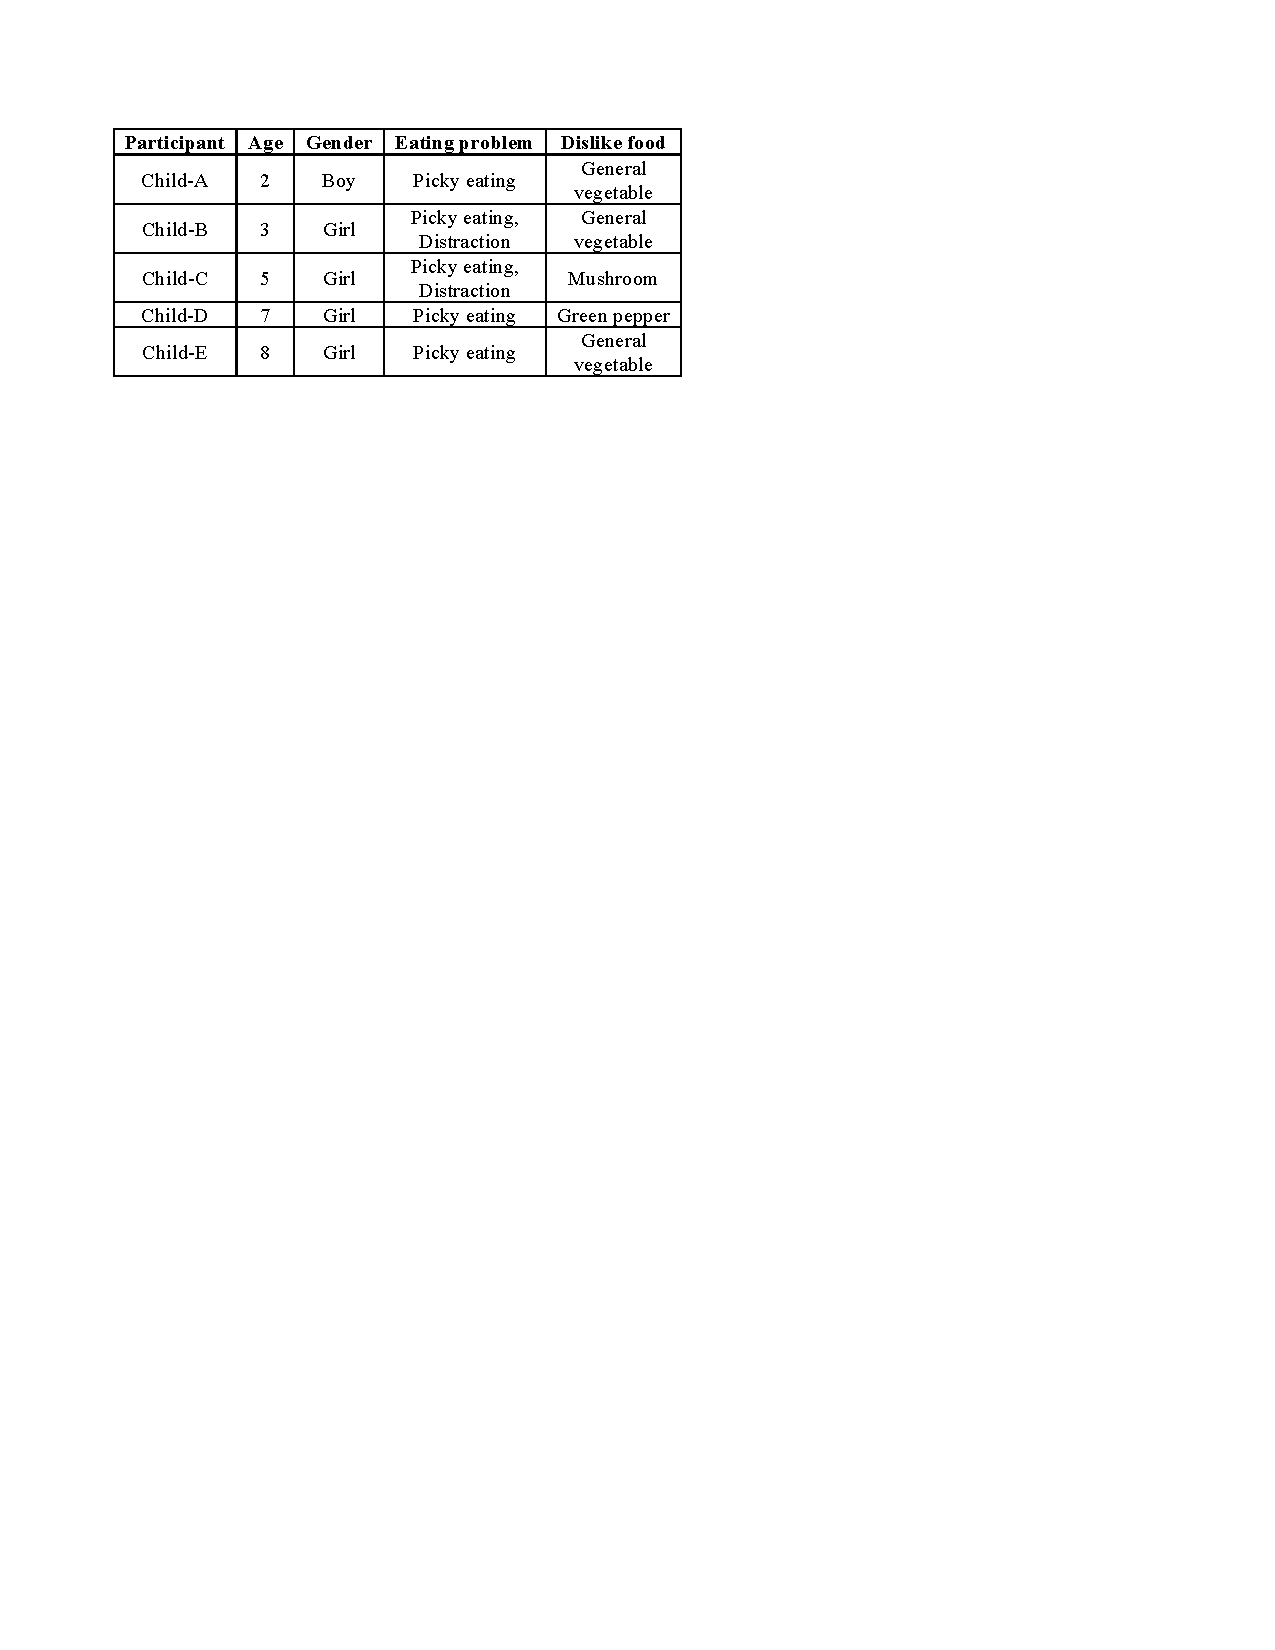
\includegraphics[width=14cm]{image/tables03.pdf}
%\caption{Details of child participants.}
%\label{table3}
%\end{center}
%\end{table}
%
%\subsubsection{Results and Findings}
%This section presents results and findings by analyzing data collected from the user study. 
%The collected data include recorded mealtime videos and semi-structured interviews 
%answered by the mothers on their experiences of the nine-day user study. 
%After transcribing the recorded mealtime videos and the interviews, 
%we coded transcriptions and organized the themes of the findings 
%based on thematic analysis \cite{Thematic:2006}. 
%
%Results from the post-meal \textbf{Question I} suggested 
%that our system made a positive impression on all mother-child pairs. 
%Results from \textbf{Question II} indicated that most children had no problem holding 
%and poking food with the Sensing Fork. 
%One noticeable exception is Child-A, who was only two years old at the time 
%and found that the fork grip was larger than he was accustomed to. 
%Despite this difficulty, Child-A was able to finish his meals using the Sensing Fork. 
%
%\begin{table*}
%\begin{center}
%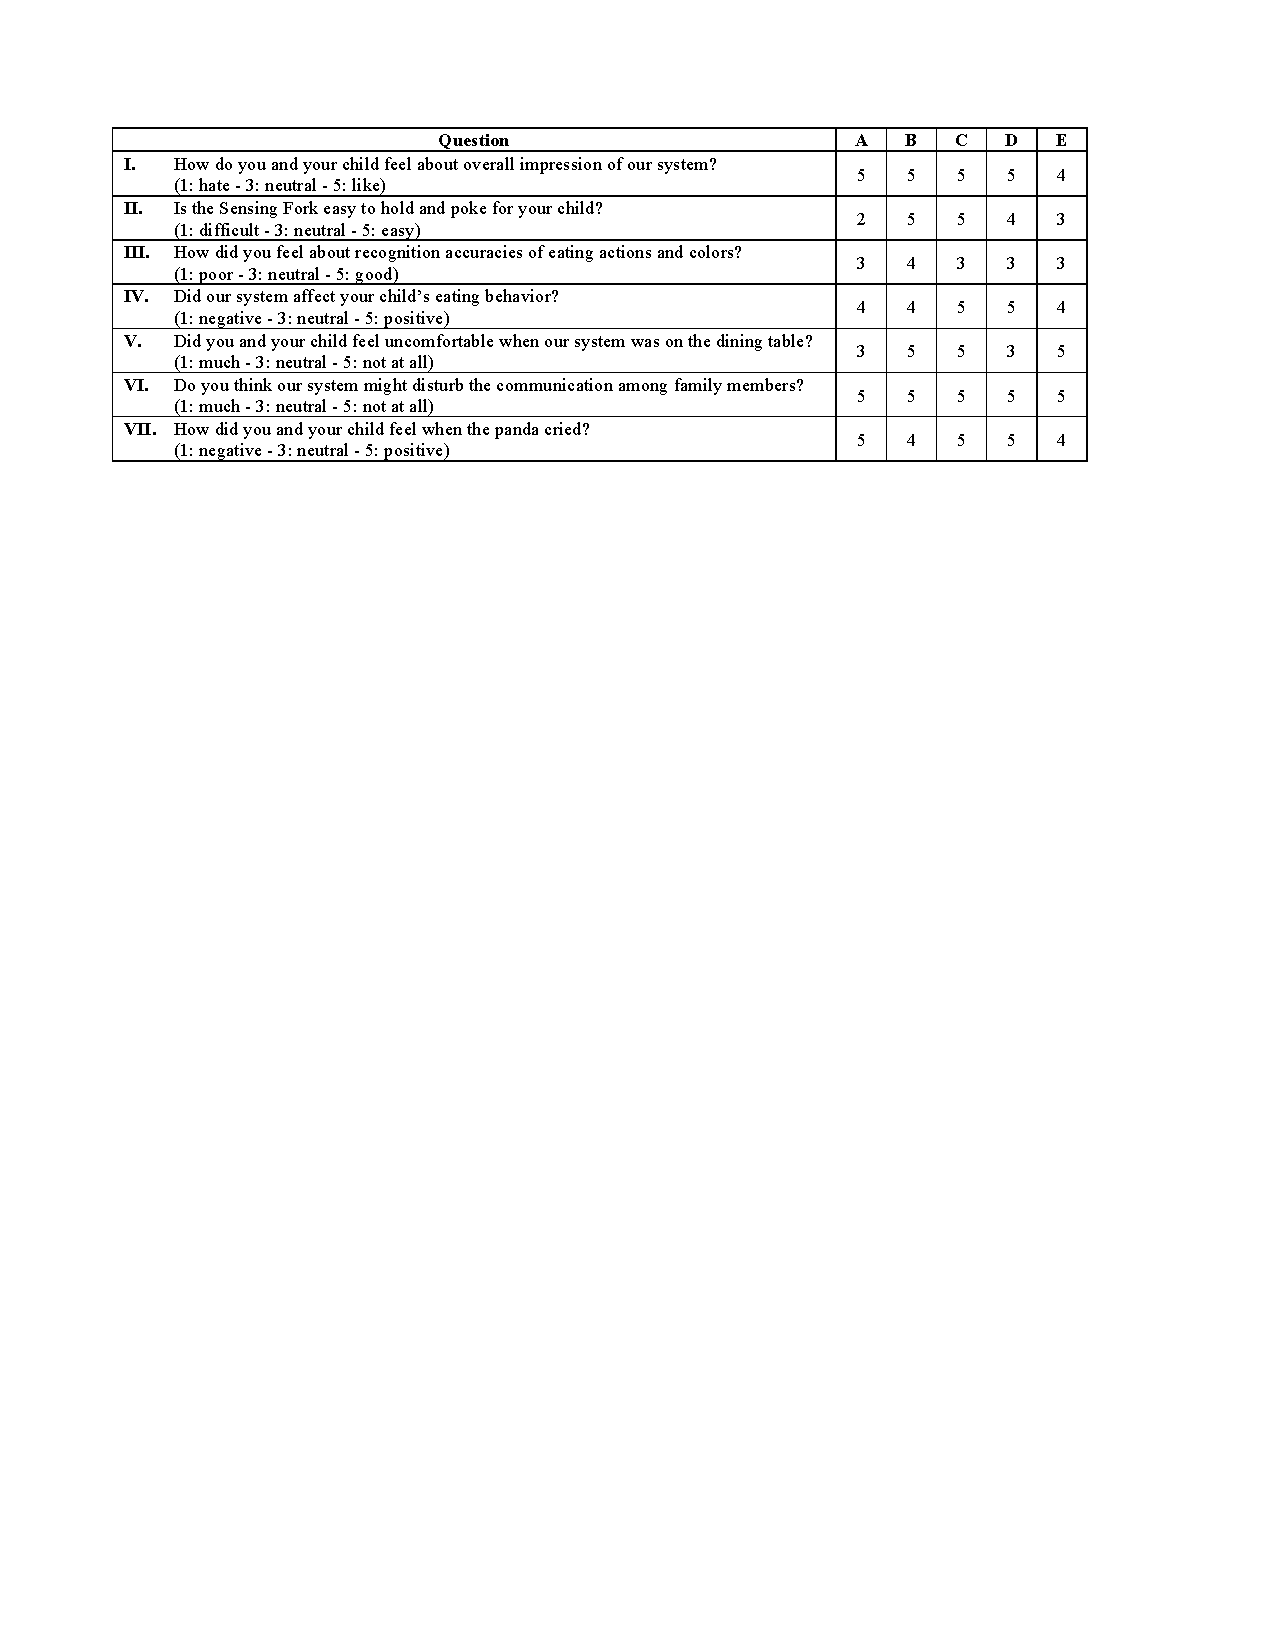
\includegraphics[width=15cm]{image/tables04.pdf}
%\caption{The results of the questionnaire in the post-meal survey (five-point Likert scale). Higher score is better.}
%\label{table4}
%\end{center}
%\end{table*}
%
%\textit{System Accuracies in the Real-World}
%\newline
%The post-meal \textbf{Question III} attempts to understand 
%how well the participating mothers perceive the fork's sensing accuracy 
%and whether it is good enough for playing the Hungry Panda game. 
%Later, we conducted semi-structured interviews to further investigate the mothers 
%on their experiences with the system's recognition accuracy. 
%All mothers said that the eating action detection was near perfect; 
%however, they observed that the food color classification was sometimes incorrect 
%and inaccurate food classification was the primary reason 
%behind their 3-4 scores in \textbf{Question III}. 
%
%To quantify the accuracy of food color classification, 
%we analyzed the recorded mealtime videos from the meal sessions. 
%A research-trained staff coded the recorded mealtime videos 
%and labeled the ground-truth food poked by children. 
%We then calculated the classification accuracy by comparing the ground-truth data 
%with the output from the food-color classifier. 
%The average food classification accuracy was 52.3\%, 
%significantly lower than the 87.5\% accuracy in the pre-study performance evaluation. 
%There were several reasons for this accuracy gap. 
%The mothers used a pre-trained classifier that is less accurate than a per-meal classifier. 
%Some children added colored seasonings to the meals, e.g., soy sauce on sashimi tuna, 
%resulting in significant color changes to the food. 
%Although mothers noticed the classification errors had an adverse effect on the system, 
%none of them reported frustration or indicated 
%that these classification errors rendered our system unusable. 
%For example, Mother-A said: \textit{``The accuracy of classifying the food color was not indispensable because Child-A only knows the names of a few colors. 
%He seemed to enjoy the panda acting the way that he did.''} 
%Mother-B and Mother-C gave similar remarks. 
%
%\begin{figure}[t]
%\begin{center}
%\includegraphics[width=14cm]{image/Mao-dish01-01.png}
%\caption{Child-C's dishes before and after of Western food days for each term.}
%\label{mao}
%\end{center}
%\end{figure}
%
%\textit{Improvement in Picky Eating}
%\newline
%Results from \textbf{Question IV} suggested 
%most children improved their eating problems than usual. 
%Table \ref{table3} shows that all participating children were picky eaters. 
%During the interviews, we asked the mothers how the Hungry Panda game affected 
%their children's picky eating. 
%Most of them responded positively. 
%For example, 
%Mother-A responded, \textit{``If we (my husband or I) encourage Child-A to eat vegetables, he almost never does. However, he ate some vegetables without our persuasion during the Hungry Panda game. Also, Child-D ate all her green pepper, something she used to hate.''} 
%Child-B was strongly disinclined to eat red pepper on the Chinese food day in Term 1 
%even her mother encouraged her. 
%However, Child-B ate red pepper in Term 2, despite disliking them. 
%Mother-C shared a similar experience: 
%\textit{``On the Western food day in Term 1, my child would not eat the mushrooms at all; however, 
%in Term 2, she ate all her mushrooms without much persuasion from me. I was very surprised. 
%In Term 3, she again ate most of the mushrooms.''} 
%%The recorded mealtime video revealed that Child-C said: \textit{``I'm starting to like the mushrooms!''}
%Figure \ref{mao} shows pictures of Child-C's Western food day 
%plate before and after meals. 
%
%These examples suggest that our system was able to 
%help children overcome their aversion to certain foods. 
%In the cases of Child-A, Child-B and Child-C, 
%their mothers noted that the reason for their children's dislike was that 
%they had never tried the food or they were turned off by the food's appearance. 
%However, we could not see remarkable effects on Child-E. 
%From the recorded mealtime videos, we observed that Child-E and Mother-E interacted 
%much less than the other participating families. 
%During mealtime, they were mainly talking 
%about daily life rather than immersing themselves in the game. 
%
%\textit{Improvement in Distraction}
%\newline
%Child-B and Child-C have a distraction problem, 
%meaning that they cannot concentrate on eating 
%and often leave the table to play with toys nearby (Table \ref{table3}). 
%Results from \textbf{Question IV} of Child-B and Child-C includes 
%their distraction problem results besides picky eating. 
%Both mothers observed that they were able to generate their children's sympathy 
%toward the Hungry Panda, as a means to persuade their children to concentrate on eating. 
%During the interview, Mother-B said: 
%\textit{``Child-B really does not like to eat, and so it always takes a long time to begin. However, during Term 2, she sat earlier than usual by the panda on the table. Moreover, the Hungry Panda picture book included her name, so this improved her interest and concentration. I could make her pay attention to the meal by saying: ``Look! The panda is crying because he is very hungry. If you eat, the panda will be happy!'' Normally, she does not listen to what I say; however I found that if I said things through the panda, she would listen.''} 
%The recorded mealtime videos revealed the following interaction 
%between Mother-C and Child-C on the Chinese food day in Term 2. 
%Child-C placed the Sensing Fork on the table for a while, and then the panda said, 
%\textit{``I want to eat more...(crying)''} 
%Mother-C said, 
%\textit{``Miss Panda wants you to eat more! Haha!''} 
%Child-C then picked up the Sensing Fork and continued eating. 
%
%These findings suggest that the Hungry Panda game 
%was successful in attracting children's attention. 
%This is vital. 
%If a game cannot attract attention and interest in the first place, 
%it is not possible to take it to the next step in persuading children 
%to improve their eating behavior. 
%
%\textit{Potential Effect of Dietary Education}
%\newline
%During the interview, we asked the mothers 
%about how effective was the system's dietary education on family member. 
%%The Hungry Panda's picture-book for dietary education provided a simple and fun introduction for teaching children about eating a balanced meal. 
%All mothers agreed that reading the picture book prior to eating a meal 
%was a natural prelude to the meals. 
%%During the interview, 
%Mother-A said: 
%\textit{``I originally thought that dietary education might be a little too difficult for Child-A. Of course, it was the first time educating him about diet, but he could pick up and understand little pieces. In addition, after nine days of reading the picture book, Child-D remembered and recited the five food colors.''} 
%Mother-A further commented: 
%\textit{``From using this system, I felt that my cooking did not have as many diverse food items as it should. I will prepare more diverse food items in the future.''} 
%%During the interview, 
%Mother-B said: 
%\textit{``Child-B cannot read and write Japanese, but she could remember the five colors during eating and tried to collect five food colors during Term 2. I could also learn the proper balanced diet by using this system. Because she has not started school yet, we did not know about dietary education.''} 
%Mother-E commented: 
%\textit{``Child-E learns dietary education at school, and she finishes all her school lunches. But at home, because I do not force her with anything, she acts spoiled and does not eat food she dislikes. The Hungry Panda game was good that she also eats such disliked foods at home as well.''}
%
%Our findings suggest that the Hungry Panda's picture book was easy to learn 
%as a dietary education tool, and it affected the behavior and mind of mother-child pairs. 
%%preferences of children. 
%
%\textit{Effect of Mobile Device at the Dining Table}
%\newline
%The post-meal \textbf{Questions V} and \textbf{VI} attempt 
%to address any potentially negative effects in having a smartphone at the dining table during meals. 
%Three mothers did not express any discomfort because they always put their smartphones 
%in a visible place in the dining place. 
%During the interview, 
%Mother-A raised a concern about the potential conflict between the TV and a smartphone during mealtime. 
%Mother-A said: \textit{``The reason for giving the score 3 on Question V is this: If mealtime includes all family members, I turn off the TV. In this case, the system may interrupt our conversation. When my children eat by themselves or alone, I turn on the TV. If the smartphone is an extension of the TV, I can accept it. Also, the Sensing Fork and Hungry Panda game provide some meaningful education, so now I like it.''} 
%Mother-C noted that smartphones were acceptable when used only as a display during mealtime: 
%\textit{``If my child touches and fiddles with the smartphone during mealtime, I will be angry. However, in Term 2, the smartphone was merely a display; therefore, I did not mind it.''} 
%
%\textit{Effect of Crying Panda as Negative Feedback}
%\newline
%The post-meal \textbf{Question VII} aims to understand 
%how participants perceive the use of the crying panda and whether 
%this negative reinforcement is counter-productive to improving their children's eating behavior. 
%Recall that the crying panda appears when a child stops eating 
%or puts down the Sensing Fork for a certain time period. 
%Questionnaire results report nothing negative about the crying panda. 
%During the interview, we investigated this question further with the mothers. 
%They responded that they did not mind the crying panda.
%
%\textit{Limitations in Feeding}
%\newline
%It is common for parents to feed very small children their food directly. 
%However, our system is not intended for assisted feeding owing to the design of the mechanism. 
%Although the panda recognizes \textbf{Holding} and \textbf{Poking}, 
%the system will not recognize \textbf{Biting} when the parent is holding the Sensing Fork; 
%hence, the child cannot gain any bamboo grass points. 
%
%From the recorded mealtime videos, 
%we found that our system has the possibility to encourage small children 
%to feed themselves owing to this limitation. 
%Mother-A (to Child-A), Mother-B, and Mother-C sometimes feed food items to their child directly. Child-C sometimes asked Mother-C to feed her. 
%However, they soon understood the system's limitation 
%because the panda did not eat the bamboo grass (and only held it). 
%Mother-C then stimulated Child-C to eat by herself, saying, 
%\textit{``If you eat by yourself, the panda will be more happy.''} 
%Following this, Child-C tried to eat by herself. 
%
%\textit{Dual Sensing Forks Scenario}
%\newline
%During the interview, 
%Mother-A stated, \textit{``Child-D wanted to reach the same bamboo grass points that Child-A had already obtained. Then, Child-D attempted to compete with Child-A.''} 
%Although we did not design our system considering a multiple-user scenario, 
%we observed this interesting interaction between Child-A and Child-D. 
%
%\subsection{Discussion}
%\subsubsection{Importance of Parental Involvement}
%Our device is not intended to replace parents and their role in rearing children. 
%Instead, our system is designed to be an assistive device 
%to help parents generate positive mealtime interaction with their children. 
%The game uses the Hungry Panda, a charming virtual pet, 
%to stimulate parent-child conversations and 
%to provide opportunities for parents to draw out children's motivation to eat. 
%For example, when Child-C put down the Sensing Fork causing the panda to cry, 
%Mother-C used this opportunity to motivate her child to eat: 
%\textit{``Miss Panda wants to eat more! Haha!''} and 
%Child-C responded positively by picking up the Sensing Fork to help the Hungry Panda. 
%In the user study, we have observed most mothers treating the game 
%as an opportunity for motivating their children to eat. 
%As an assistive device, our system should not offer excessive feedback 
%that may draw too much attention to the game, 
%interfering with parent-child interaction. 
%We observed that if a child interacted with our system without parental involvement, 
%our device was not effective for improving eating habits. 
%
%\subsubsection{Use of Negative Feedback} 
%Although prior works \cite{Consolvo:2008}\cite{Lin:2006} cautioned against 
%the use of negative feedback, 
%suggesting that it may adversely lose the user's drive for behavioral change, 
%results from our user study indicate that mothers did not mind the negative aspects 
%in the crying panda. 
%As a matter of fact, mothers were able to use the opportunities presented 
%by the crying panda to stimulate their children to eat. 
%We believe that there is some space for the use of negative feedback with children, 
%and that negative feedback ought to be designed carefully 
%to mitigate any undesirable effects. 
%In our case, the negative effect of the crying panda 
%is only temporary ---rapidly switching to positive feedback, 
%a happy panda, when the child again picks up the Sensing Fork. 
%This rapid switch from negative to positive feedback encourages children 
%to want to improve their eating habits in order 
%to fulfill their desire help the Hungry Panda. 
%
%\subsubsection{Multiple-user Scenario}
%We believe that a multiple-user system can capitalize 
%on children's competitive attitude to further enhance motivation. 
%However, multiple-user competition may not work for very young children 
%as most children develop competitive attitudes 
%at around the age of four \cite{Priewasser:2013}. 
%Our user study involved a two-children scenario. 
%We observed competitive tendencies in the eight years old, Child-D, 
%but not in the two years old, Child-A.

\subsection{Limitations}
\textit{Food Classification: Pre-trained or Per-meal Classifier:}
A pre-trained classifier provides low food-classification accuracy 
but requires no user effort to train the classifier. 
A per-meal classifier provides high food-classification accuracy 
but requires some user effort to train the classifier. 
In consideration for the parent, we adopted a pre-trained classifier 
in the real-life user study ---hence the negative feedback 
from the mother respecting classification error. 
To reduce the effort involved in training a per-meal classifier, 
we have created a step-by-step tool in the application 
with which a parent can poke each food sample in his/her child's meal multiple times 
using the Sensing Fork. 
Upon completion, the application will automatically send the food-sample data 
for training and build a meal-specific classifier. 
\vspace{10pt}
\newline
\textit{Fork, Spoon and Other Utensils:}
\newline
To eat food such as soups or stews, a spoon is a more appropriate utensil than a fork. 
It is possible to reuse the design for the Sensing Fork and apply it 
for building other Sensing Utensils. 
For example, motion sensors embedded in a Sensing Spoon can recognize spoon actions. 
A pair of electrodes can be used to distinguish liquid from solid food, 
because liquids have a lower resistance value than solids. 
\vspace{10pt}
\newline
\textit{Game Application Design for Persuasion and Education:}
\newline
With repeated use, children may become weary of an unchanging picture book and game. 
However, because the picture book and game are mobile applications, 
it is relatively easy for users to download new educational content 
in the picture book and/or update the Hungry Panda game 
with a new game that a child has not yet played. 

\subsection{Summary}
In this study, we implemented a sensor-embedded eating utensil called the Sensing Fork 
for detecting a user's eating behavior (eating actions and food colors). 
As a sample application compatible with the Sensing Fork, 
we designed the Hungry Panda game targeting children's eating behavior. 
The aim of the Hungry Panda game was to address children's eating issues, including picky and distracted eating. 
Embedding the sensing technology into a conventionally-used item 
is more acceptable to the children if persuasive education tools are included in daily life.
\newpage









\section{Enabling Daily Self-monitoring to Assist Recovery from Drug Addiction through a Phone-based Support System}

Drug addiction has long been recognized as one of the most challenging social problems facing society. Drug use poses health risks, such as drug over-dose and exposure to HIV infection and other blood-borne diseases, and also leads to crime and poverty. Seriously drug-dependent patients commonly are forced to enter rehab centers for treatment; however, individuals returning to daily life face renewed temptations that often lead to relapse. Previous studies \cite{addiction_relapse_rates} have reported that 40\% to 60\% of the patients leaving rehabilitation programs relapse. An on-going support system is often necessary to help patients exert control over their behavior, increase their self-efficacy, and encourage them in maintaining abstinence. Support systems, such as cognitive behavior therapy (CBT), involve the self-monitoring of one's own drug-use behavior. This self-monitoring approach enables users to track and assess their progress, enhance their awareness regarding the need for behavior changes, and give them the confidence required to overcome addiction.

Several monitoring systems and screening kits have been developed for the detection of drug usage; however, they have a number of shortcomings, including: (1) the need for costly specialized equipment, (2) limited to specific environments, (3) vulnerabilities to cheating (4) lack of personalized data collection and feedback support. No existing system is able to overcome all four of these shortcomings. The Alere DDS MobileTest System \cite{Moore2013} uses a specialized handheld device with a test cartridge to screen for drug usage; however, this system costs several thousand dollars and is tailored to law enforcement for the roadside drug screening of drivers. The intelligent fingerprinting system \cite{MobileDrugTesting} is a portable device capable of analyzing a tiny quantity of sweat from fingerprints in detecting traces of drug metabolites. It essentially minimizes the likelihood of cheating; however, the costly device is several thousand US dollars \cite{drugfingerprint}. Numerous cost-effective FDA-approved drug test kits are now available in grocery stores. Most of them use membrane strips \cite{drugscan,drugwipe} coated with chemicals that react to the presence of drug metabolites in urine or saliva. Unfortunately, the collection of urine samples requires access to a private bathroom and saliva-based systems are susceptible to cheating, when performed anywhere except under supervision in a drug test center.

\begin{figure}[ht]
\begin{center}
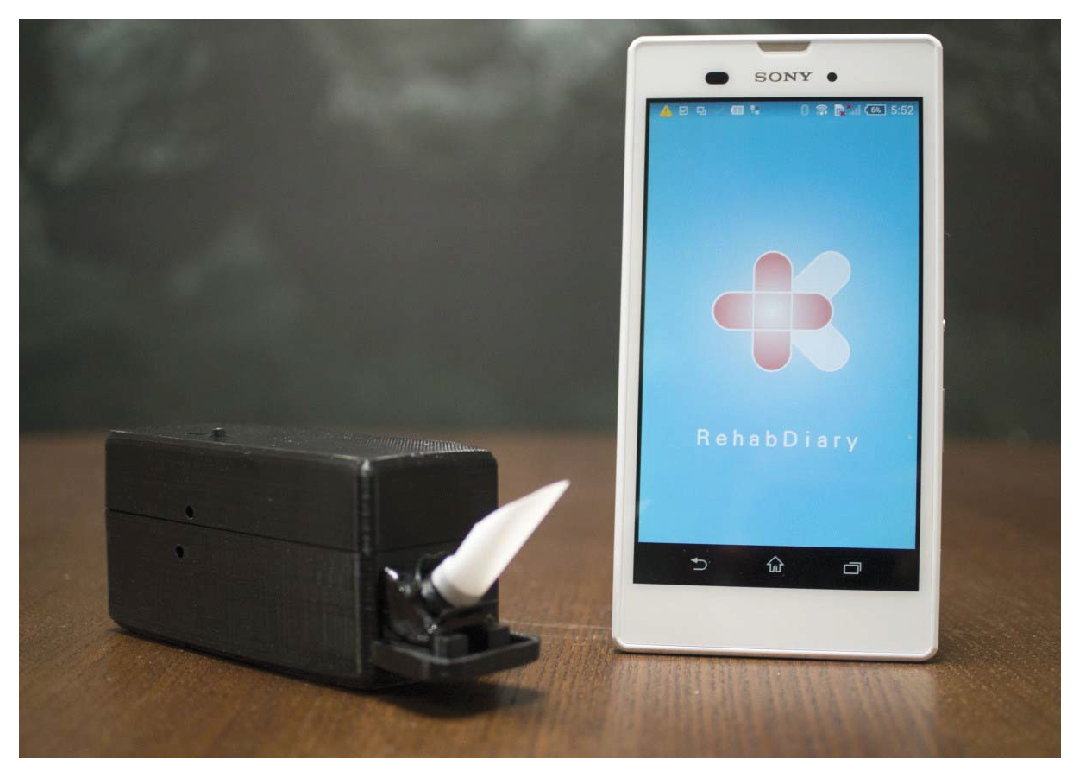
\includegraphics[height=5.8cm]{image/ket/concept_photo.eps}
\caption{Proposed system for daily self-monitoring of drug use, comprising saliva screening device and mobile smartphone.}
\label{fig:overview_photo}
\end{center}
\end{figure}

The RehabDiary system (Figure \ref{fig:overview_photo}) proposed in this study leverages the capabilities of smartphone to reduce the system costs, thereby making the devices available to even those from a low socio-economic background. Drug testing can be also conducted anywhere and the built-in smartphone application provides a cheating-prevention mechanism as well as personalized data collection, progress-based feedback, and motivational support.  Furthermore, the proposed system provides the same degree of accuracy as any test strips used in existing FDA-approved drug test kits.

In this study, we targeted a schedule III controlled substance \cite{ketamine_schedule_III}, ketamine, which poses a moderate to low potential for physical and psychological dependence and is an emerging drug of choice among students, particularly in East and South-East Asia \cite{WorldDrugReport}. In 2010, ketamine users accounted for 1.7\% of the general population of the UK, making it the fourth most popular of the so-called club drugs \cite{Morgan2012}. Note that our system design is generalizable to self-monitoring other types of drugs, such as amphetamines, cocaine, ecstasy, marijuana, opiate, etc., which have inexpensive test strips.


\subsection{System Overview}

\begin{figure}[ht]
\begin{center}
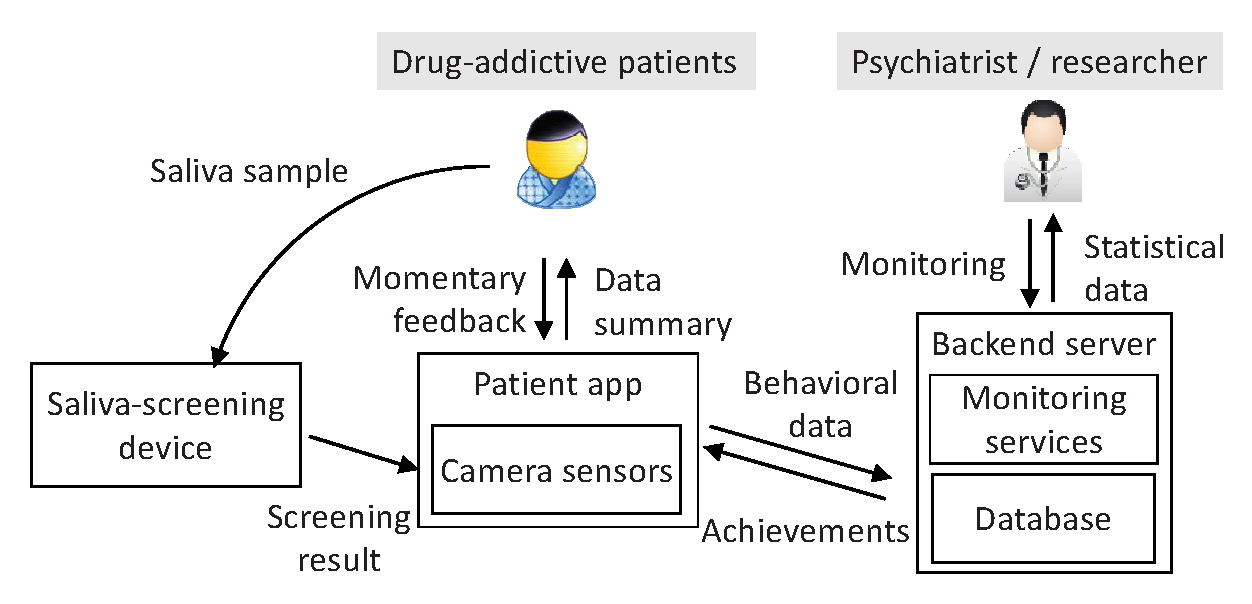
\includegraphics[height=6cm]{image/ket/arch.eps}
\caption{The system architecture.}
\label{fig:system_overview}
\end{center}
\end{figure}

Figure \ref{fig:system_overview} shows the RehabDiary system, which consists of a portable Bluetooth saliva-screening device, a smartphone app, and a backend server. Phones that senses participants' drug-use behavior. Patients start a saliva screening test by inserting a replaceable cassette into a customized screening device. Once the patient initiates a saliva test, the phone carried by patients installed with the RehabDiary phone application automatically connects with the screening device via Bluetooth and examines the validity of the cassette. To make sure that it is the patient and not someone else taking the test, the patient is required to show his/her face using the screening device in front of the phone camera. After the strip is soaked by patient's saliva, the app waits ten minutes for the test strip to absorb the saliva, during which time the patient can browse through the app's psychiatrist-provided coping skills. At the end of 5 minutes wait, the phone app identifies line patterns appearing in the reaction zone of the strip and notifying patients of the results, which are also uploaded to a backend server for future analysis. 
These components are described as follows.

\subsubsection{Saliva-screening Device}
Figure \ref{fig:overview_photo} shows the saliva-screening device, which facilitates patients to collect their saliva and screens patient's ketamine use. Before each test, patients simply plug in a replaceable and single-use test cassette, which contains a saliva test strip \cite{saliva_test_cassette}.  After the strip interacts with absorbed saliva, the camera sensor inside will photograph the image of the strip. All images will send back to the phone to further analyze the screening results appearing on the strip.
%In the next section, the detailed design and implementation will be described.
%Figure 1(a) shows the saliva-screening device and a replaceable, single-use test cassette. Compared to urine and blood screening, saliva screening [14] is easy-to-use, involving no blood or lavatory trips. Patients simply spit saliva into a straw on the saliva-screening device (Figure 1(a)), which contains a customized sensor board equipped with a TI CC2541 microcontroller [2] and an off-the-shelf camera module [3]. The microcontroller triggers the camera module to capture images of the test strip's reaction zone. Once the microcontroller receives this image from the camera, it has a Bluetooth radio to transmit images to the patient's smartphone. Between the camera and the reaction zone, three white LEDs are used for illumination. Before taking a test, patients simply clip a single-use test cassette into the opening of a device. Figure 1(b) shows a single-use test cassette printed with a 3D printer. Inside the test cassette are a saliva test strip (with a cutoff sensitivity of 50 ng/ml) [5] and an auxiliary circuit board containing an Atmel AT24C01D EEPROM [4], a micro USB connector, and two pairs of conductive pads. To ensure the integrity of each screening test, a unique ID is associated with each cassette. After patients spit saliva into the device's straw, it flows over the strip through a small saliva drain. A pair of conductive pads on each end of the strip detect saliva absorption. When saliva absorption reaches a threshold and over a certain time period, it triggers the camera to take several images of the reaction zone. Photos and saliva absorption readings are then sent back to the smartphone for processing. 


\begin{figure}[ht]
\begin{center}
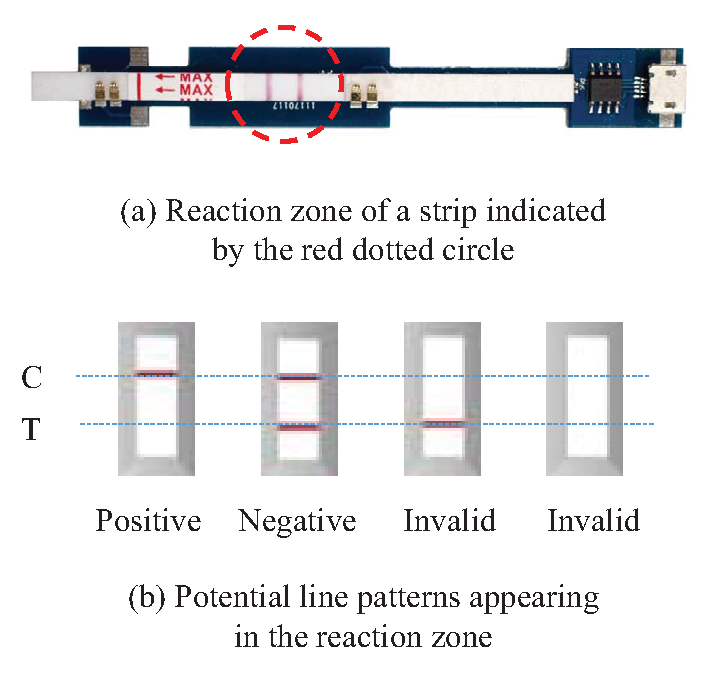
\includegraphics[height=8cm]{image/ket/line_pattern.eps}
\caption{The reaction zone of a strip and its potential line patterns. ``C'' (``T'') means the control (test) line of the pattern.}
\label{fig:line_pattern}
\end{center}
\end{figure}

\subsubsection{Phone Application}
The RehabDiary phone application (1) enables ketamine-dependent patients to self-monitor ketamine use with saliva tests, (2) summarizes their progress in maintaining abstinence, and (3) incorporates face recognition techniques to prevent cheating. To increase patient awareness of ketamine use behavior through self-monitoring, this application processes the photos of the test strip sent from the screening device to  detect if the test outcome is negative (two lines), positive (one control line), or invalid (no control line) in Figure \ref{fig:line_pattern}(b). To visualizes patients' progress of ketamine abstinence as an immediate feedback of their daily usage, the application shows the phone app notifying patients of the results, which are also uploaded to a backend server. Since this patient population tends to cover up their drug use with lies, we ask patients to take multiple photos of their frontal faces. The application will compare the features of the frontal face with those collected when setting up the application. 


\subsubsection{Backend Server}
The backend server records test results and patients' feedback sent from the phone application. These records can be further summarized for psychiatrists to review or sent back to patients' phones for their progress assessment and encouragement.

\subsection{Saliva Screening Design}
\label{sec:design_of_saliva_screening}


\begin{figure}[ht]
\begin{center}
\includegraphics[height=7.7cm]{image/ket/device_photo.eps}
\caption{Electrical components on the circuit boards and connections between boards.}
\label{fig:device_photo}
\end{center}
\end{figure}

The proposed saliva screening system comprises two components: a saliva-screening device and a smartphone application. Excretion of ketamine into the saliva enables detection even one or two days after ingestion \cite{saliva_test_cassette}. The app reminds the patients to perform at least one saliva test per day to enable the screening of ketamine before it is metabolized by the liver. In the following, we describe the hardware used in the collection of saliva samples for the screening of drug metabolites using off-the-shelf saliva strips \cite{saliva_test_cassette} loaded into a replaceable test cassette. The cassette sends data to the smartphone via Bluetooth for processing by the app. In the following, we outline the design of the hardware and software components, including  hardware, firmware, and the smartphone application.


\subsubsection{Portable Saliva-screening Device}
Figure \ref{fig:device_photo} illustrates the proposed saliva-screening device, comprising a \emph{portable} screening module and a \emph{replaceable} cassette that holds test strips. After spitting saliva into a straw for drug-use screening, the test cassette can simply be disposed of, without the need to clean the device.

\textit{Portable screening module:}
\newline
Figure \ref{fig:overview_photo} presents a side-view of our portable screening module into which the user inserts a cassette holding the test strips. The screening module tracks the operational state of the inserted cassette and captures a photograph of the line patterns that emerge in the reaction zone.

The main board (Figure \ref{fig:device_photo}(a)) is connected vertically to the secondary board (Figure \ref{fig:device_photo}(b)) through a 5-pin header to enable tracking of the operational state of the cassette, such as whether the strip in a cassette is ready for detection or whether it has been previously used. When a cassette is inserted into the screening module, the device interfaces with a small memory device in the cassette in order to retrieve the unique identification number associated with each cassette. An off-the shelf camera module is mounted in a fixed position within the device to enable the capture of a photographic of the the line patterns emerging in the reaction zone of the test strip. Monochromatic light emitting diodes (LEDs) surround the lens of the camera to function as a light source to illuminate the reaction zone.

%\begin{figure}[ht]
%\begin{center}
%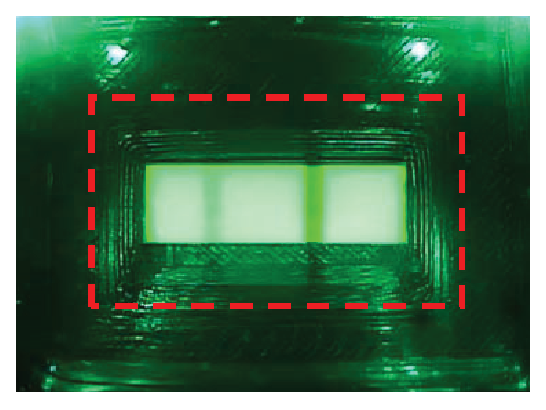
\includegraphics[height=8cm]{image/ket/cassette_photo.eps}
%\caption{Photo captured by on-board camera. The red-dotted rectangle indicates the area in which test patterns appear. The inner red rectangle indicates the pattern window in the potential area. }
%\label{fig:cassette_photo}
%\end{center}
%\end{figure}

Figure \ref{fig:all_color} presents images of the reaction zone captured by the camera when illuminated using monochromatic LEDs of (a) green, (b) blue, (c) red, and (d) white, showing luminance values as measured in the R, G, and B channels. In the RGB color model \cite{Forsyth:2002:CVM:580035}, subtractive colors are seen when pigments in an object absorb particular wavelengths of white light while reflecting the rest. The placement of a Red, Green, or Blue filter in front of the image sensor does not eliminate all wavelengths outside the monochromatic spectral region \cite{s8117300}. This results in the generation of cone-shaped spectral sensitivity curves, colored conjugated antibodies (the reagent) \cite{dasgupta2011health} interact with then chemical coating in the control line or test line. 
An improper light source would reduce the likelihood of correctly classifying line patterns as being positive or negative when few amount of reagent accumulates in the test line.
Thus, in this study, a green LED provided the clearest rendering of the test strips.

\begin{figure}[ht]
\begin{center}
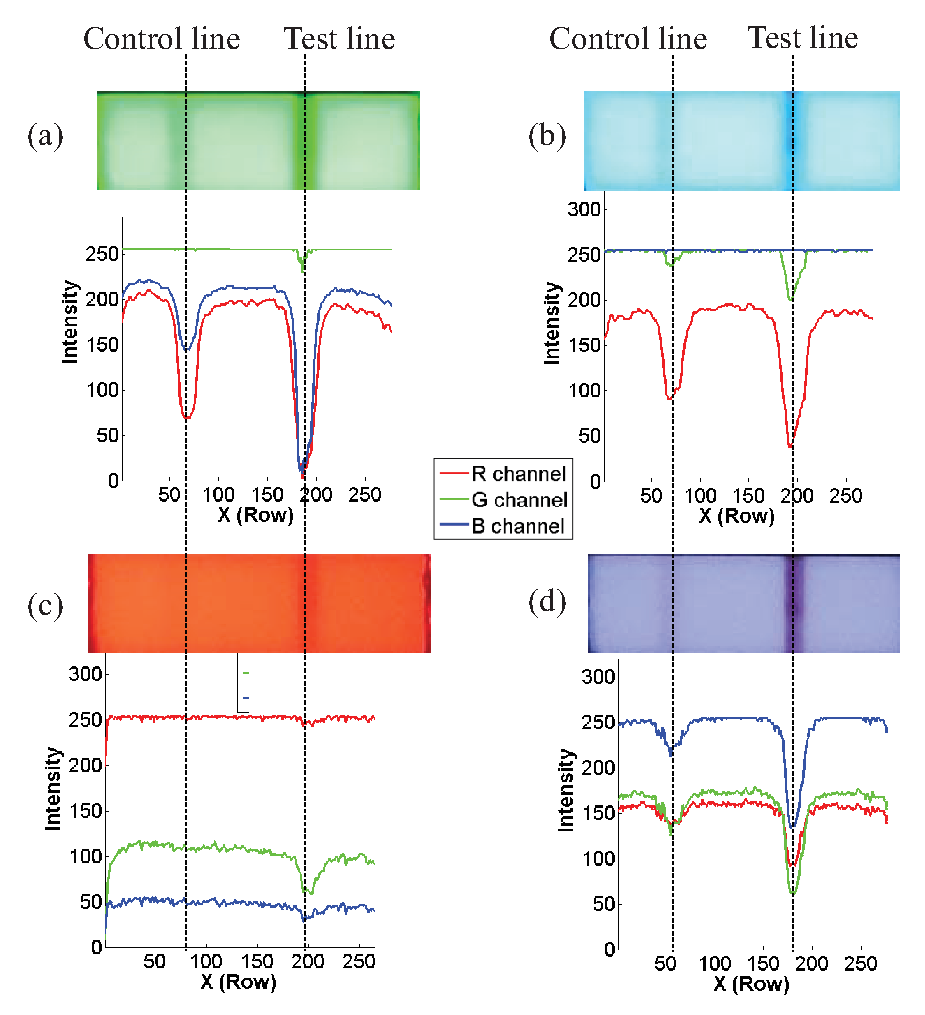
\includegraphics[height=12cm]{image/ket/all_color.eps}
\caption{Image of reaction zone illuminated using monochromatic LEDs: (a) green, (b) blue, (c) red, and (d) white. The RGB readings across the middle row of pixels in the image are plotted as a line chart below each image.}
\label{fig:all_color}
\end{center}
\end{figure}

\textit{Replaceable test cassette:}
\newline
Figure \ref{fig:device_photo}(c) presents a replaceable test cassette with an embedded auxiliary board enclosed within upper and lower cases. During each drug test, the patient spits saliva into the cassette, after which it is simply thrown away. Because the units are meant to be disposable, we used inexpensive components for the nonvolatile memory, micro-USB connector, spring fingers \cite{springfinger}, and testing strip and adopted surface mount manufacturing techniques for assembly. Non-volatile EEPROM memory is also mounted on the board to store the unique ID for each cassette. As shown in Figure \ref{fig:device_photo}, two pairs of spring fingers are placed at the front and back end of the strip to hold the absorbent cotton wick of the test strip, thereby forming an electrical component with infinite resistance (Figure \ref{fig:equivalent_circuit}(b)). These two equivalent resistances ($R_1$ and $R_2$) and a high load resistance ($R_3$ = 1M Ohms) form a voltage dividing circuit. By interfacing with the main board through the micro USB connector, the microcontroller makes it possible to obtain data from the cassette.

\begin{figure}[ht]
\begin{center}
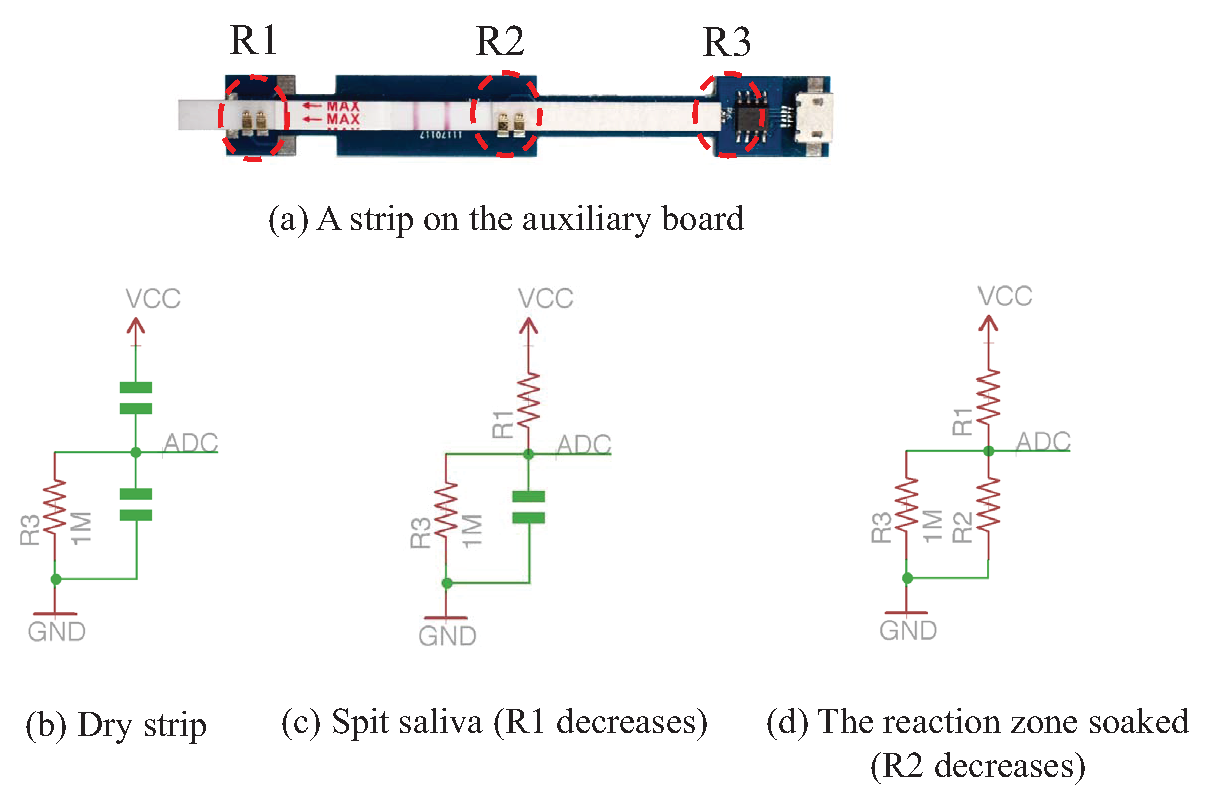
\includegraphics[height=10cm]{image/ket/equivalent_circuit.eps}
\caption{Auxiliary board with test strip and three equivalent circuits. When the strip is dry, the equivalent circuit (b). Saliva samples are absorbed by the front cotton wick resulting in equivalent circuit (c). When the back cotton wick is also soaked, the equivalent circuit is in (d).}
\label{fig:equivalent_circuit}
\end{center}
\end{figure}

\textbf{Cassette state sampling:}
\newline
The status of each test cassette is monitored by relaying data related to the saliva absorption and screening to ensure their integrity. These actions are performed after receiving state transition commands from the app. Briefly, the device retrieves the ID number of the cassette, samples the voltage of the dividing circuit, and captures an image of the reaction zone.

\emph{ID retrieval}:  Unique ID identifiers prevent the falsification of saliva samples through the insertion of previously used cassettes. Throughout the test, the device periodically retrieves the ID number from EEPROM to ensure that the cassette is not removed.

\emph{Voltage sampling}: After reading the ID number, the screening device engages in continuous sampling of the voltage across $R_3$ (Figure \ref{fig:saliva_absorb}) via the USB connector. Figure \ref{fig:equivalent_circuit} presents three equivalent circuits associated with the cassette. In the case where the strip is dry, the resistance values of the cotton material overlaid on the strip ($R_1$ and $R_2$) are nearly infinite, such that the current does not pass $R_3$ (Fig. \ref{fig:equivalent_circuit}(a)). Figure 9(c) shows the equivalent circuit in which the front end of the strip soaked with saliva. Figure \ref{fig:equivalent_circuit}(d) shows the equivalent circuit in which the front and back ends of the strip are soaked with saliva. Establishing profiles pertaining to the sequences of voltage samples makes it possible for the system to determine whether the saliva sample has been provided correctly


\emph{Photo capturing}: The microcontroller communicates with the camera using a serial protocol to record the line patterns appearing in the reaction zone of the test strip. Following the collection of saliva and confirmation that both ends of the strip are soaked, the app waits for 5 minutes to enable a reaction with chemicals embedded within the reaction zone of the test strip. The microcontroller then sends a command to the camera to acquire a photo of the reaction zone after receiving a shooting command from the app on the smartphone. 
Finally, the ID, voltage samples, and captured images are sent to the app for processing.

\begin{figure}[ht]
\begin{center}
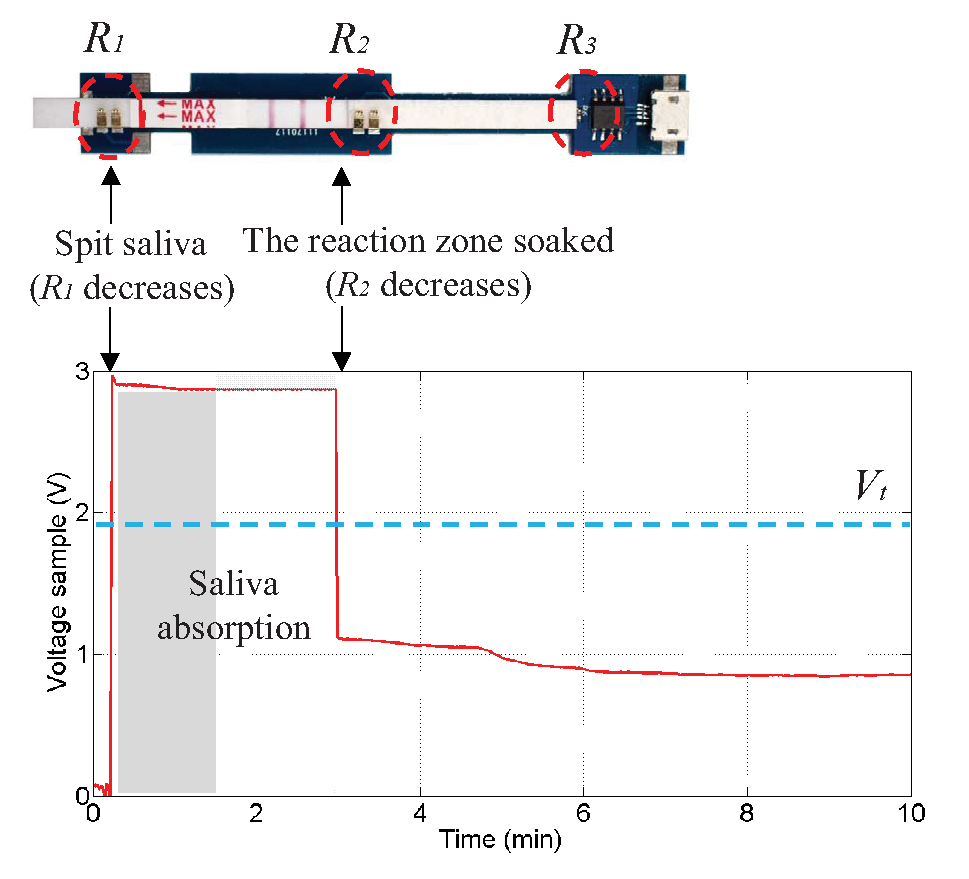
\includegraphics[height=9cm]{image/ket/saliva_absorb.eps}
\caption{Voltage samples of determining saliva test progress.}
\label{fig:saliva_absorb}
\end{center}
\end{figure}


\textbf{Line pattern classification pipeline:}
\newline
After receiving images from the screening device, the smartphone app performs analysis in three steps: (1) window localization, (2) control pattern validation, and (3) test pattern classification.

\emph{Window localization: }
In this step, pixels within the pattern window are identified in order to locate the reaction zone of the strip. Manufacturing the upper casing of each test cassette using a 3D printer leads to differences in the expansion and contraction of the PLA material, which can alter the location of the pattern window by 5 $\sim$10 pixels. Thus, we included a window localization step to frame the exact position of the pattern window. The color contrast between the pattern window (green) and the outer casing (black) is significant; therefore, the pattern window can be identified by selecting light-colored pixels in the estimated locality of the pattern window. In this manner, we can determine the location of the pattern window by finding the upper-left and lower-right corners, i.e., \{$x_{ul}$, $y_{ul}$\} and \{$x_{lr}$, $y_{lr}$\}, of a box bounding the over-exposed pixels.

\emph{Control pattern validation: }
The proposed algorithm scans one half of the reaction zone row-by-row in order to validate the screening results. No control line emerges when the screening result is invalid. Based on the location of the pattern window, we can extract each row within the pattern window by searching for a dip in the intensity of the R channel in order to identify the control line. After reviewing all of the patterns collected, we determined that the intensity of the control line was always lower than that of the test line. Figure \ref{fig:row_by_row} plots intensity in the R channel across one row of pixels. Based on this sharp control line, we designed a heuristic detection algorithm for the detection of the control line in each row. We first search for a significant decrease in intensity in the control line by identifying the position of the lowest dip in each row. The location of the control line can then be pinpointed by calculating the average positions of all dips. with the average column of all dips. Once the location of the control line has been determined, the region of the test line (test region), can be located by assuming that the distance between the control and test lines is constant. Identifying the lowest dip in the test region makes it possible to pinpoint any position in the test line. Most of the reagent accumulates along the control or test line; therefore, the curve presents two dips; i.e., a dip in the intensity values of the control and test lines with a flat area between the two dips. To characterize the drop in intensity associated with the two dips, we respectively calculate the average intensity in the control region, test region, and flat area, i.e., $I^c$, $I^t$, and $I^f$, respectively. The \emph{control (test) drop} of the control (test) dip can be defined as the difference between average values of the control (test) line and the flat area, i.e., $D^c$ ($D^t$). One row is used as a part of the control row only when the dip in the control region is large enough to be differentiated from smaller noisy disturbances; i.e., $D^c_i > S^f_i$. Otherwise, the row is not recognized as a part of the control line. Therefore the score of a $i$th row can be defined as the follows.
\begin{equation}
\label{eq:row_detect}
\text{V}_i = \begin{cases}
1, &\mbox{if } (I^w_i - I^t_i) = D^c_i > S^f_i \\
0, &\mbox{otherwise }
\end{cases}
\end{equation}
where $V_i$ is the contributing score of row $i$ as the control line. By summarizing the scores of all the rows, the screening results can be considered valid when the total score is larger than half the total number of rows.


\begin{figure}[ht]
\begin{center}
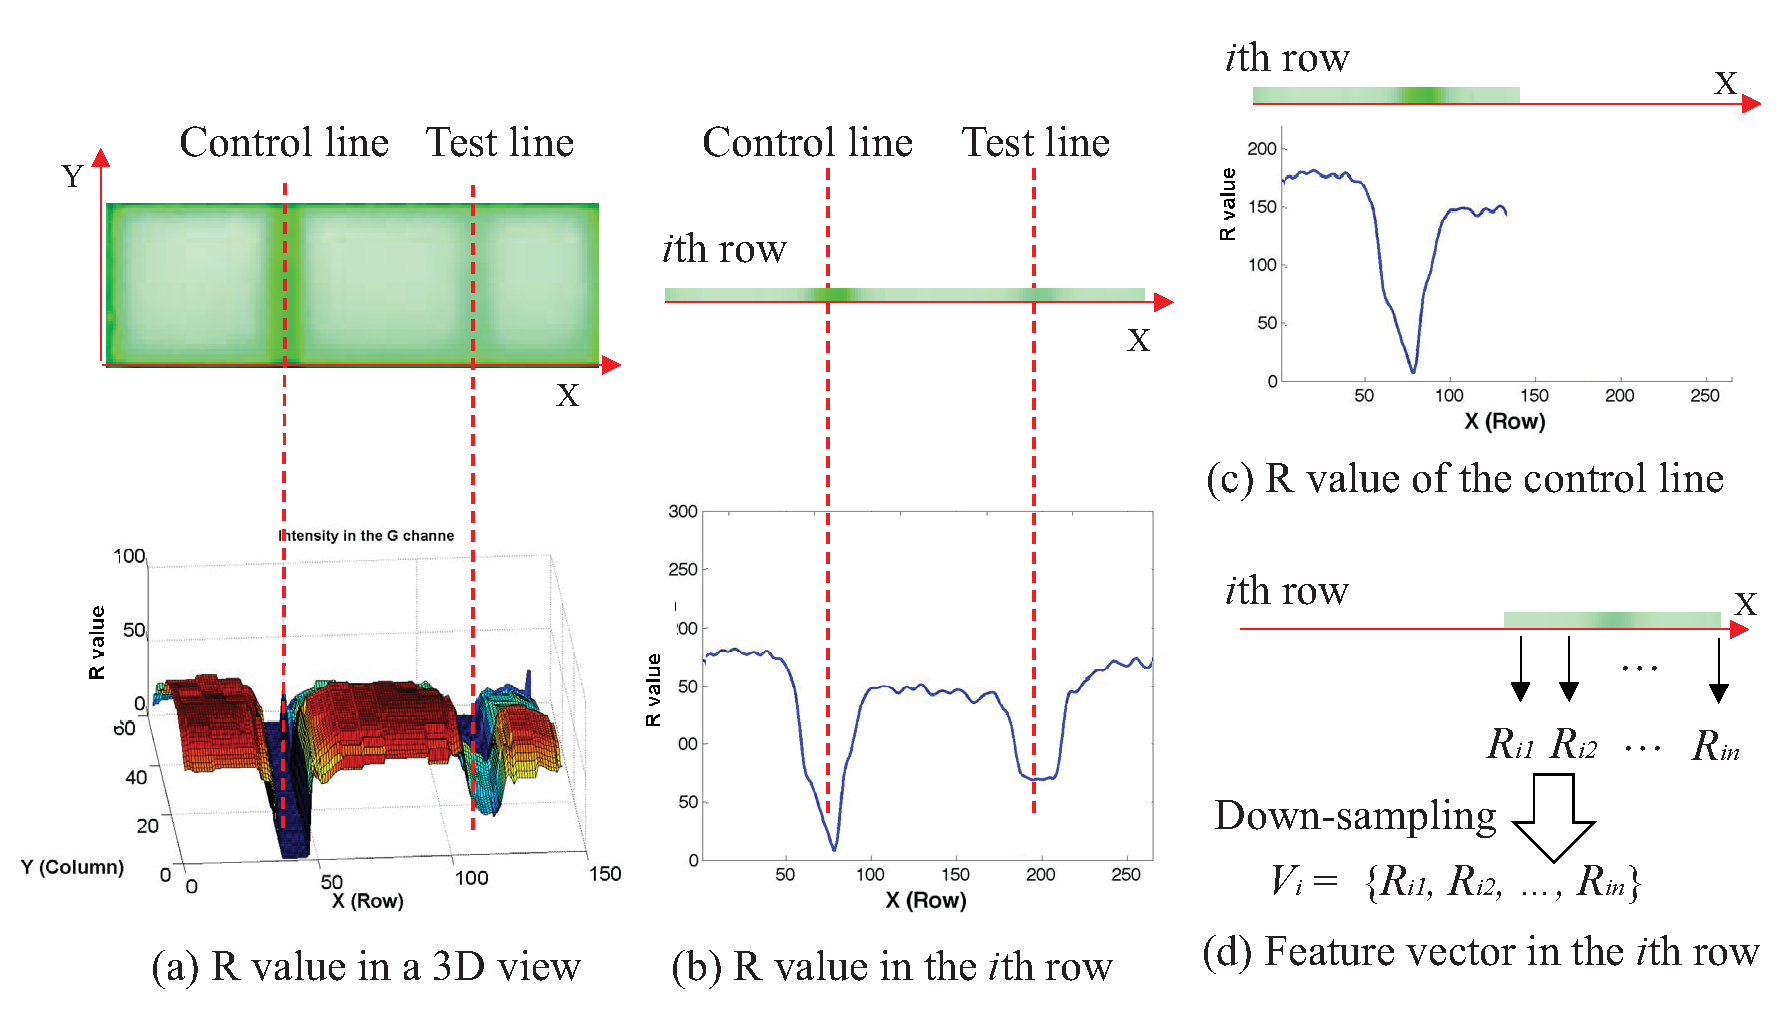
\includegraphics[height=8.5cm]{image/ket/row_by_row.eps}
\caption{The row-by-row intensity analysis while validating the control line and classifying the test line.}
\label{fig:row_by_row}
\end{center}
\end{figure}

%
%\begin{figure}[ht]
%\begin{center}
%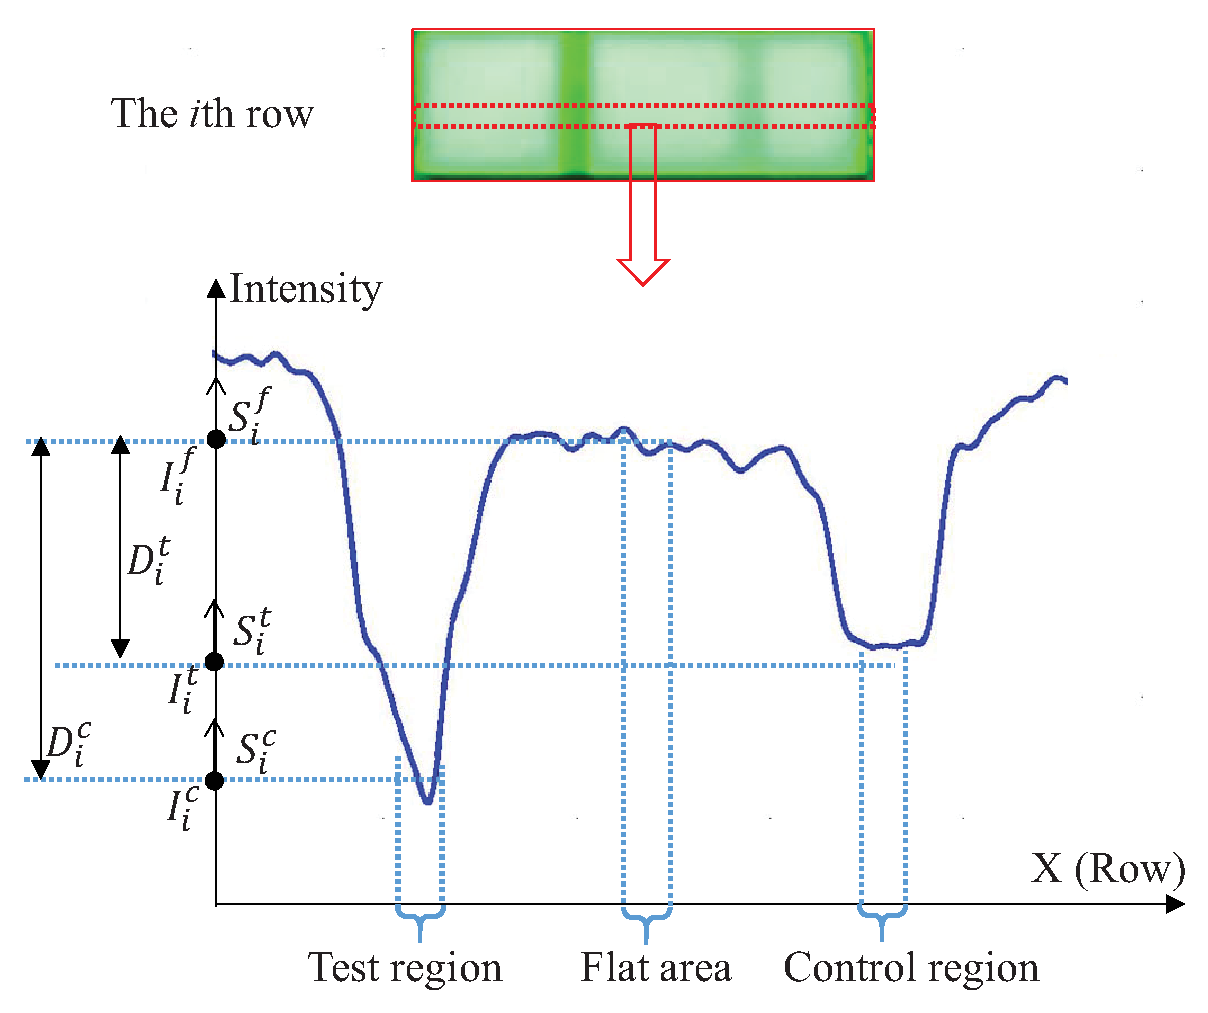
\includegraphics[height=8cm]{image/ket/delta.eps}
%\caption{Differences among control region, test region, and flat area in the $i$th row.}
%\label{fig:energy_delta}
%\end{center}
%\end{figure}


\emph{Test pattern classification: }
Following validation of the screening results, the patterns in the test line are classified as positive or negative. The quantity of magenta reagent that attaches to the test line varies according to the amount of the target drug ingested by the patient. The accumulation of the magenta marker influences the intensity of green light reflected back to the camera. The heuristic algorithm used to detect the test line may fail to identify lines with a slight magenta color; therefore, we implemented a learning algorithm to facilitate the accurate classification of all test lines as either positive or negative line patterns.

The system crops out half of the image to prepare the input feature vector associated with the test line pattern in the pattern window (Figure \ref{fig:row_by_row}(d)). The system then down-samples the intensity values in the R, G, and B channels of each row and concatenates all three sequences of R, G , and B values together to form an input vector of the pattern. We also normalize each component using the svm-scale tool \cite{Chang:2011}. Feature selection is performed on the training set to enable the selection of a feature subset of arbitrary size, which best characterizes the statistical properties of the given target classes based on the ground truth labels. The final step of classification involves the use of a support vector machine (SVM) \cite{Chang:2011} for the classification of  all of the pattern lines as either positive or negative. Using the selected feature subset, the SVM is trained to predict the class label of each line pattern in the test set.

\textbf{Cassette validation processing pipeline:}
\newline
Validating the testing operation involves the processing of ID data and voltage samples from the screening device to ensure that the current cassette is unused that the patient has performed saliva collection as prescribed.


ID data is compared with an ID number downloaded from the server to ensure that a valid cassette has been inserted. Verifying that saliva collection is performed correctly involves checking the sequence of voltage samples to ensure that the changes in voltage proceed as expected. Figure \ref{fig:saliva_absorb}(a) presents the voltage readings recorded during the saliva collection phase. The high resistance of the absorbent cotton wick on the strip means that the resistance between adjacent spring fingers ($R_1$ and $R_2$) is infinite, as shown in Figure \ref{fig:equivalent_circuit}(b). Thus, the voltage across the load resistance ($R_3$) is pulled down to ground (0V).


Saliva that soaks into the cotton wick slightly decreases resistance at $R_1$, which pulls up the supply voltage of the regulator along the conductive path formed by $R_1$ and $R_3$ to a value close to 3 volts, as shown in Figure \ref{fig:equivalent_circuit}(c). With the further absorption of saliva into the cotton wick on the other end of the strip results in resistance values at $R_2$ comparable to that at $R_1$, as shown in the 3$rd$ minute in Figure \ref{fig:saliva_absorb}. Figure \ref{fig:equivalent_circuit}(d) shows the resulting equivalent circuit when the strip is soaked at both ends, in which the decrease in $R_2$ lowers the equivalent resistance between the sampling point and the ground, which results a voltage drop to below the given threshold ($V_t$) of 2 volts in this study. 

\subsection{User Interface}
The user interface is used to summarize the patients' drug use and summarize their progress in maintaining abstinence. The system is based on various behavioral theories, self-efficacy theory \cite{Bandura1994} and cognitive behavior therapy (CBT) \cite{Volkow2011}, which are commonly used to help drug dependent patients remain abstinent. We also introduced a mechanism to prevent cheating in order to reinforce the validity of testing. Through self-monitoring, participants show their determination to exert control over their behavior and thereby increase their self-efficacy. The review of drug use logs helps them to recognize drug cravings for which they should develop strategies to cope. The smartphone application can be altered to enable the screening of different drugs as well as the mandatory screening frequency in accordance with the rate at which patients metabolize a given drug. In this study on ketamine, we set the screening frequency at one test each day in order to avoid undue inconvenience.
Self-efficacy theory to increase patient awareness of ketamine use behavior through self-monitoring [21], cognitive behavior therapy (CBT) to emphasize triggers and coping strategies to prevent relapses [19], and self-determination theory to internalize the motivation for recovery [9]. 
The smartphone app (Figure \ref{fig:phone_ui}(b)) provides four functional modules: (1) daily saliva screening, (2) screening results (3) event logging and (4) ranking of risky scenario.  

%By examining the validity of information generated by the cassette, the smartphone application can ensure that patients do indeed collect saliva and helps to prevent patients from falsifying saliva samples by inserting a previously used cassette. Facial recognition technology enables the system to alert system supervisors of cases in which other people perform the test for the patient. After completing the tests, the smartphone application presents a visual representation of the patients' progress in remaining drug-free as a form of immediate feedback related to daily usage. The smartphone application also summarizes the time and outcome of each test in a dashboard located at the top of the feedback page (Figure \ref{fig:phone_ui}(b)).

\begin{figure}[ht]
\begin{center}
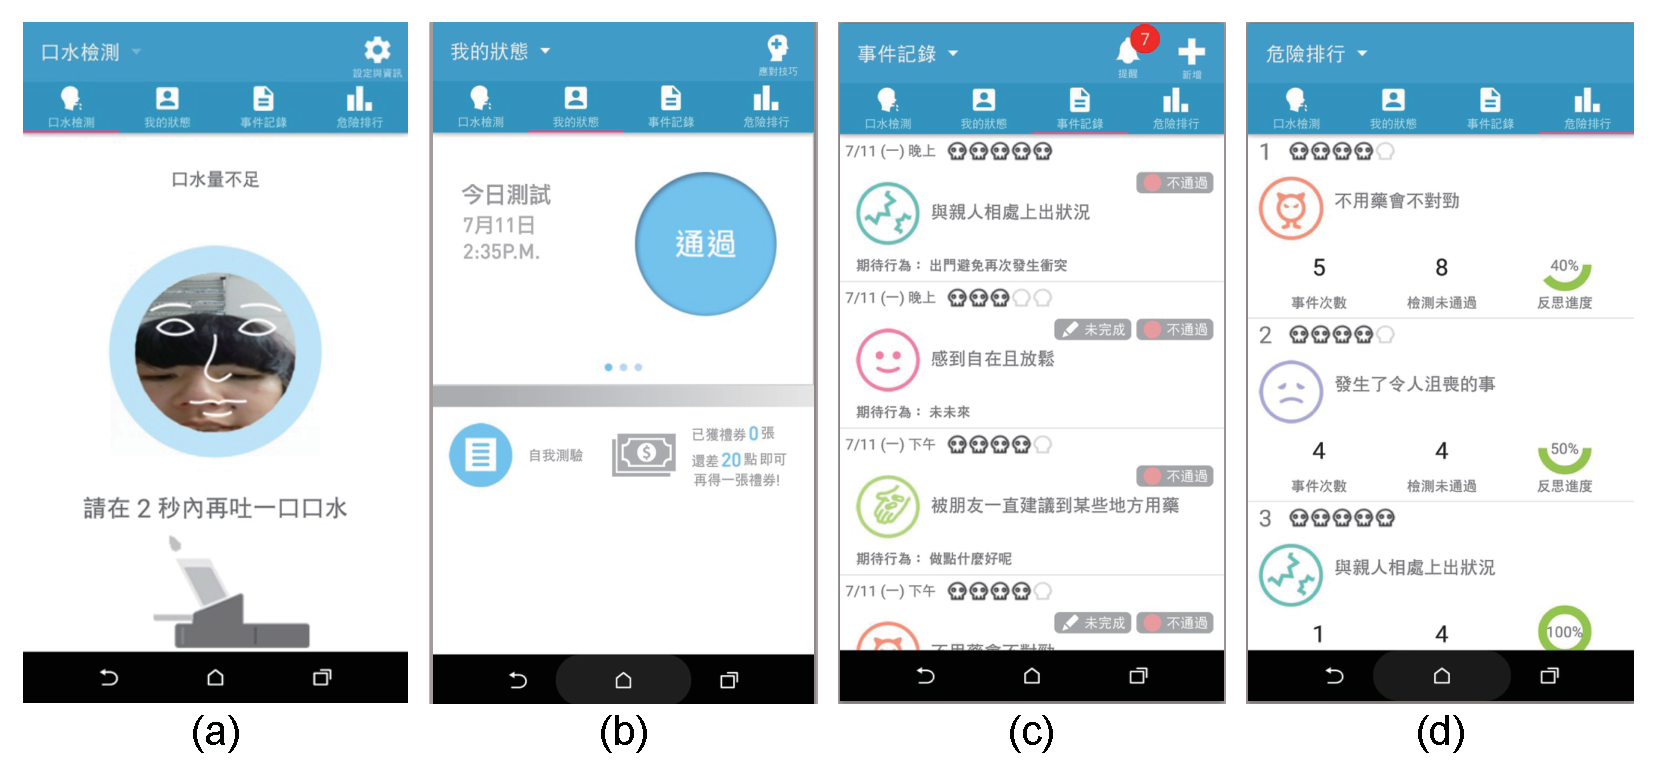
\includegraphics[height=6.9cm]{image/ket/ket_app}
\caption{User interface of smartphone application: (a) saliva screening, (b) screening results, (c) event logging and (4) ranking of risky scenario.}
\label{fig:phone_ui}
\end{center}
\end{figure}

\subsubsection{Classification Accuracy in the Recognition of Line Patterns}

To evaluate the accuracy of the proposed system in recognizing line patterns, we recruited patients from the Taipei City Psychiatric Center (TCPC) who were believed to be the most likely to test positive for drug use. This sample included outpatients who visited the hospital to seek treatment for ketamine use as well as inpatients who had recently started receiving treatment. These users commonly attempt to hide their ketamine use; therefore, they were asked to take urine as well as saliva tests in screening for positive samples. Ketamine differs in its effects on urine and saliva as well as in the rate of metabolization; therefore, the results of urine testing were adopted as the ground-truth and the results of saliva testing were accepted only in cases where they agreed with the urine tests. Images of the reaction zone were obtained only when both the saliva and urine tests were positive. Researchers and graduate students who passed urine tests were recruited to provide negative samples for the saliva test. A total of 128 negative samples and 80 positive samples were obtained.

\begin{figure}[ht]
\begin{center}
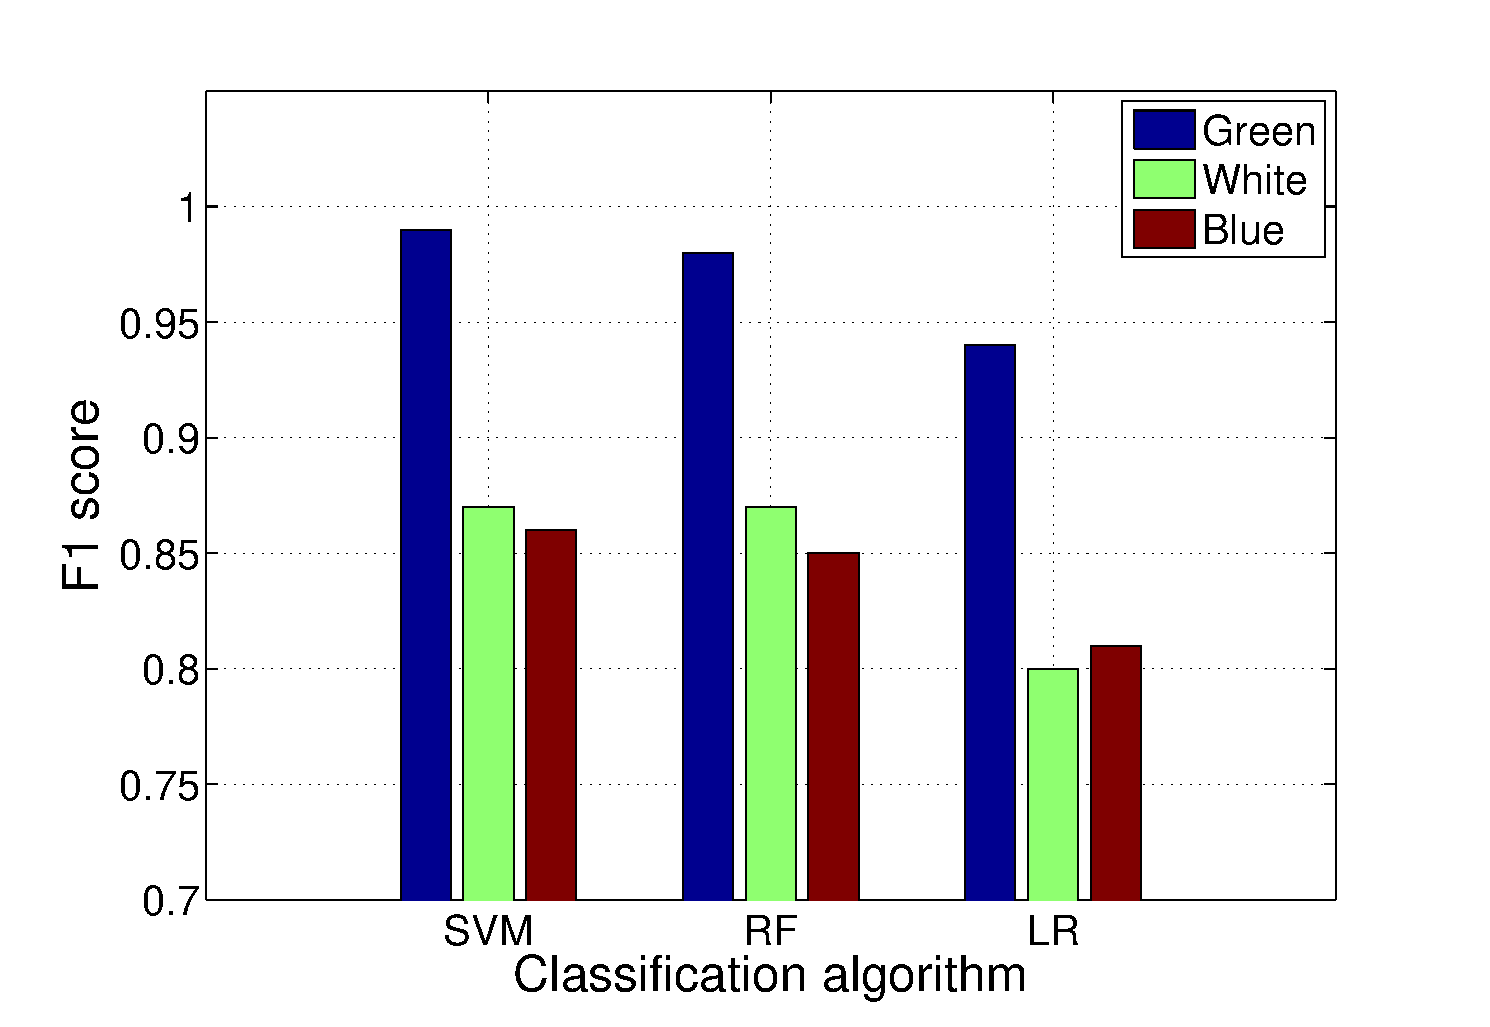
\includegraphics[height=6cm]{image/ket/detection_accuracy.eps}
\caption{F-measure accuracy of three learning classification algorithms (SVM, RF, and LR).}
\label{fig:detection_accuracy}
\end{center}
\end{figure}

Following the collection and manual labeling of samples, we followed a leave-one-set-out scheme for evaluation. The data was divided into ten randomly distributed groups, with one group serving as testing data and the other nine groups serving as training data. For the classification line patterns, we compared the accuracy of support vector machine (SVM), random forest (RF) and logistic regression (LR) ported them to run on the android smartphone. Figure \ref{fig:detection_accuracy} presents the mean F-measure accuracy results obtained under green illumination, which indicated that SVM provides the highest accuracy in the classification of line patterns (0.99) followed by random forest (0.87) and logistic regression (.80). Changing the light source to a blue (white) LED reduced the overall accuracy to 0.86 when using SVM, due to a decrease in the $avg\_delta$. Our experiment results demonstrate the efficacy of the proposed system in providing robust, accurate results in the screening of drug use.

\subsection{Summary}
This study reports the design and implementation of a cost-effective and cheating-prevention daily drug self-monit\-oring system. A saliva-screening device transmits data wirelessly to a mobile smartphone for analysis of drug use. The system also uses ID validation and image capture to prevent cheating.
In this study, ketamine was selected as a target drug; however, the saliva-screening device could be applied to other drugs simply changing the saliva test strip \cite{drugscan}. The screening device could also be extended as multi-panel screening to deal with multiple drugs in a single saliva test. Our results demonstrate the accuracy and efficacy of the RehabDiary system as a low cost alternative to drug testing.

\let\cleardoublepage\clearpage
